% Wired into report/report.tex via % Wired into report/report.tex via % Wired into report/report.tex via % Wired into report/report.tex via \input{../src/Davide/Final/Latex/assignment3.tex}
% -- report.tex already has graphicx/float in its preamble, and a shared
% report/b.bib for \cite{} (matching assignment_1's convention). All
% \includegraphics paths below are relative to report/, same as
% assignment_1/ass1.tex's own figures.

\section{Assignment 3}

\subsection{Introduction}
This assignment extends the damped wave simulator from parts 1--2 with
color. The physics, discretisation, and MPI/OpenMP structure are
unchanged: three MPI ranks each run one independent scenario (a single
impulse; two impulses starting together; two impulses with the second
delayed to $N/7$), each parallelised with OpenMP. What changes is the
output stage: each timestep's matrix is sent to the GPU, mapped to an RGB
triplet per pixel by a CUDA kernel, and saved as a P3 (ASCII) PPM frame
instead of a grayscale PGM. Bright, saturated colors mark the wave's
extrema, colors fade along the rising/falling fronts, and calm (near-zero)
regions are rendered white. 

%Student parameters (352165): $\gamma=0.067$,
%$c=0.59$, primary impulse at $(M/2,M/2)$ with amplitude 56; sim2's second
%wave at $(2M/3,M/4)$, amplitude $-35$, $t_{\mathrm{start}}=0$; sim3's second
%wave at $(M/3,M/3)$, amplitude 58, $t_{\mathrm{start}}=N/7$.
\subsection{Architecture}
The three MPI
ranks \cite{sanchezmpiintro} map naturally onto the three required
scenarios: each rank owns a complete, independent grid and runs one
scenario end to end, so the only collective call needed is a final
\texttt{MPI\_Allreduce} on success/failure. Within each rank, \texttt{compute\_next}
(the same 5-point Laplacian stencil as parts 1--2 -- each point's next
value is computed from itself and its 4 orthogonal neighbors via central
differences) is parallelised with OpenMP \cite{slidestatic}, using
\texttt{schedule(static)} for the same NUMA first-touch reason argued in
part 1: with a fixed thread-to-row mapping, the memory each thread first
writes (and therefore where the OS physically places it) matches the
memory that same thread repeatedly accesses on every subsequent call. After each timestep, the rank sends its
matrix to the GPU \cite{sanchezcuda}: a kernel normalizes each value
against the frame's own peak magnitude (found via a GPU-side reduction
\cite{sanchezgpuintro}), maps it to a color (white near zero, fading to
bright red/orange for positive values and blue for negative, saturating
at the wave's extrema), and the result is written to disk as an ASCII
PPM frame while the original scalar matrix continues to drive the
simulation.
Because the job requests a single GPU (\texttt{--gres=gpu:1}) for all
three ranks, the GPU is a shared resource -- a design point this report
returns to in Section~\ref{sec:contention}.

\subsection{Cluster hardware}
All experiments ran on Politecnico di Torino's HPC@PoliTO cluster
(Legion), specifically its EDU partitions -- reserved for coursework,
as opposed to the open-access or research-group-restricted partitions
also present on the cluster. Of the four EDU partitions, only two have
GPUs: \texttt{edu\_a40} and \texttt{edu\_v100}, confirmed live via
\texttt{sinfo -o "\%P \%D \%G"} (the other two, \texttt{edu\_skylake}
and \texttt{edu\_sapphire}, are CPU-only). \texttt{edu\_a40} nodes have 2 physical CPU sockets, 24 physical cores
per socket (48 physical cores/node), doubled to 96 logical cores/node by
SMT (2 hardware threads per core) -- confirmed via \texttt{sinfo}'s
socket/core/thread fields, since the cluster's own documentation lists
only the 48 physical cores -- and 4$\times$A40 GPUs;
\texttt{edu\_v100} nodes have 32 cores and 4$\times$V100 GPUs. Both are
used in this report: \texttt{edu\_a40} for all main results, and
\texttt{edu\_v100} as a cross-hardware check in Section~\ref{sec:nsys}.

\subsection{Metrics and the grid-size sweep}
\label{sec:metrics}
Beyond wall-clock time, the program times two phases directly:
\texttt{color\_time} (GPU colorization + PPM write, per frame) and
\texttt{compute\_time} (the OpenMP stencil update). \texttt{color\_time}
is further split into five sub-phases -- H2D copy, kernel, D2H copy,
ASCII formatting, and disk write -- introduced in
Section~\ref{sec:phase}. Figure~\ref{fig:size} sweeps grid size $M$ from
128 to 4096 (\texttt{edu\_a40}, 4 threads, 50 steps). Execution time
approaches ideal $O(M^2)$ scaling as $M$ grows: $128\to256$ costs only
$2.1\times$ (fixed per-run overhead still dominant at small $M$), while
$2048\to4096$ costs $4.1\times$ -- essentially the ideal quadratic ratio.
The right panel shows GPU colorize+write dominating total time
throughout: at $M=4096$ it is $\sim$97.6\% of total time, versus
\texttt{compute\_next} at $\sim$2.4\%. Both phases are $O(M^2)$, so this
ratio stays roughly constant across the whole sweep ($\sim$97.6--97.7\%
from $M=256$ upward; only the smallest grid, $M=128$, deviates, where
fixed per-run overhead is large enough to matter).

We capped the sweep at $M=4096$ rather than matching part 1's $M=15000$:
at $M=4096$ an ASCII PPM frame is already $\sim$100--130MB, so scaling to
$M=15000$ -- $(15000/4096)^2\approx13\times$ the pixels -- would push
single frames into the multi-gigabyte range across 50 steps and 3 ranks,
for a sweep whose purpose (showing execution time approach ideal
$O(M^2)$ scaling and locating the point where GPU colorize+write comes
to dominate) was already unambiguous well before $M=4096$.

\begin{figure}[h]
    \centering
    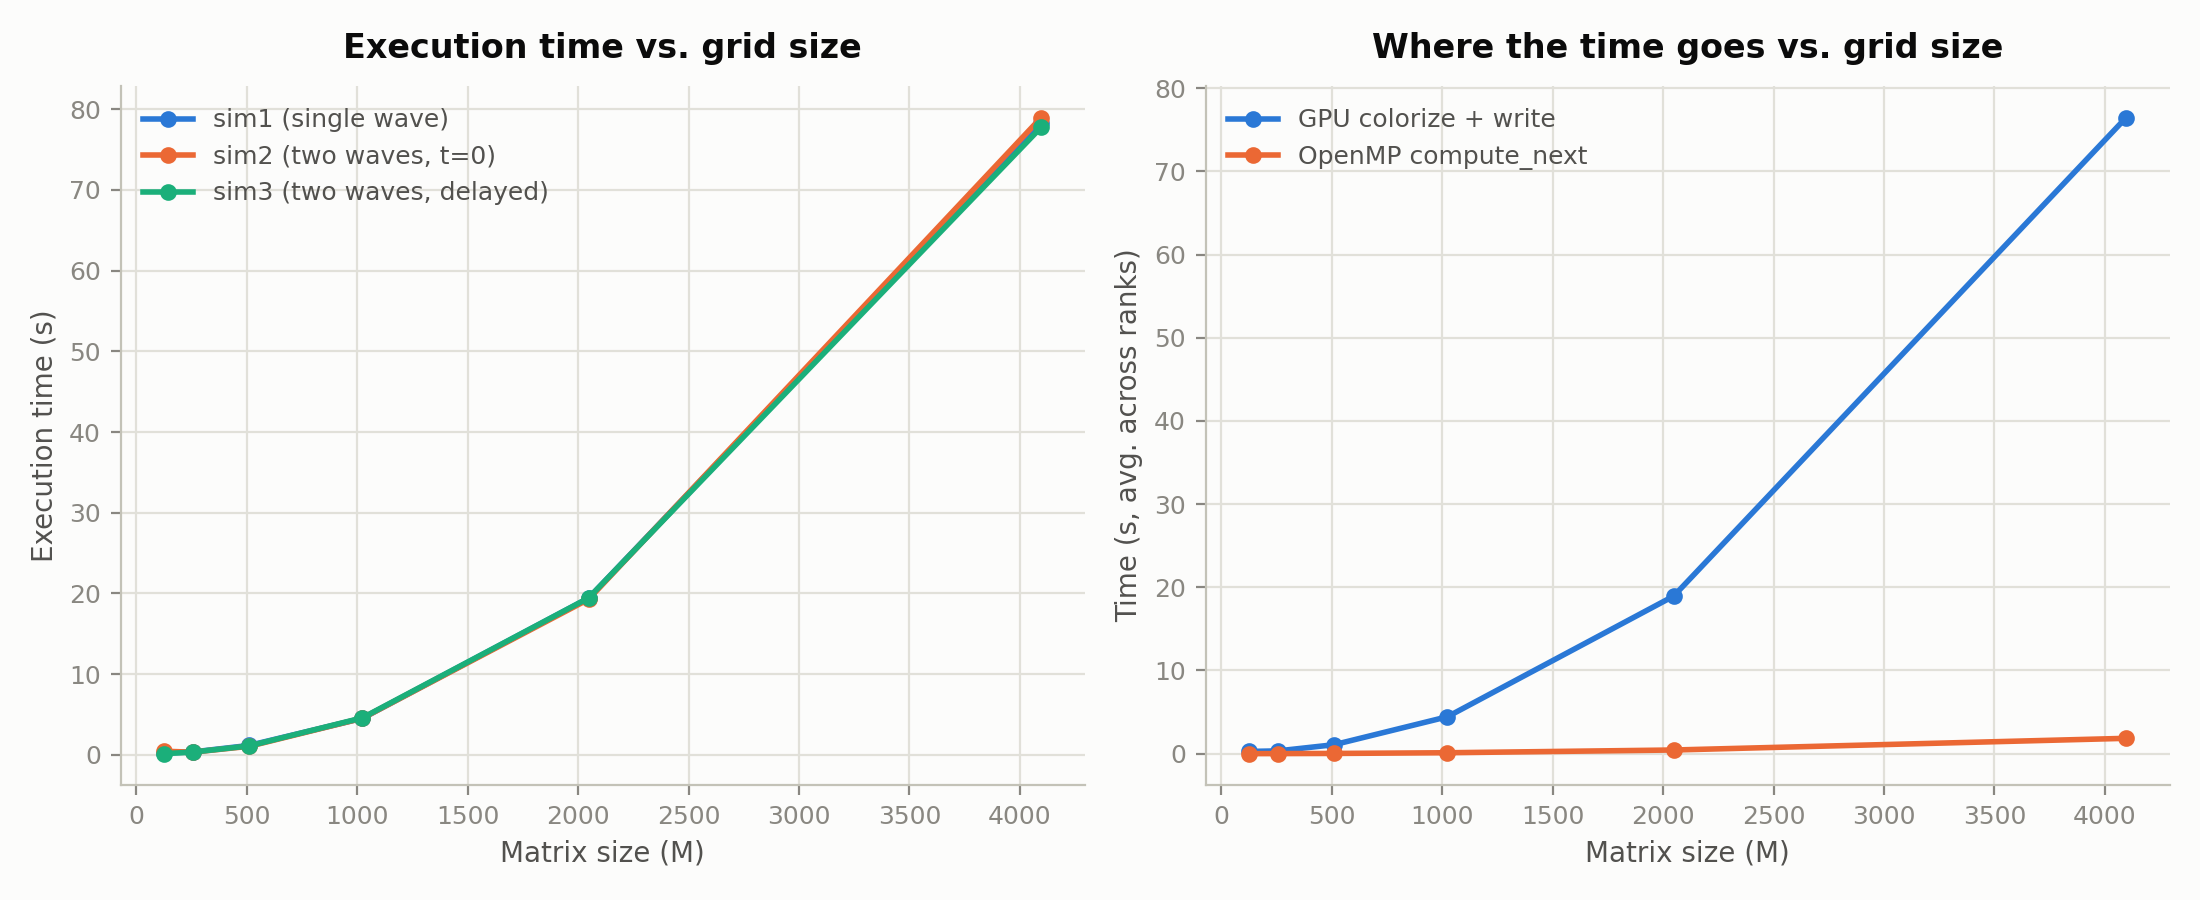
\includegraphics[width=0.68\textwidth]{../src/Davide/Final/Latex/figures/size_sweep_execution_time.png}
    \caption{Execution time and its GPU/OpenMP split, varying grid size $M$ (4 threads, 3 ranks sharing 1 GPU).}
    \label{fig:size}
\end{figure}

\subsection{Phase breakdown: is the ASCII formatting worth parallelizing?}
\label{sec:phase}
Figure~\ref{fig:phase} breaks \texttt{color\_time} into its five
sub-phases. At $M=4096$ (averaged over 3 ranks): \texttt{write} (the
\texttt{fwrite} call) is $\sim$94.6\% of \texttt{color\_time},
\texttt{format} (the ASCII byte-to-digit conversion) is $\sim$4.3\%, and
H2D copy + kernel + D2H copy combined are $\sim$1\%. The same lopsided
pattern holds at every grid size swept, not only at $M=4096$.

This directly answers a question we considered early on: is it worth
parallelizing the ASCII-formatting step with OpenMP? It is not --
formatting is only $\sim$4\% of \texttt{color\_time}, so even a
theoretical zero-overhead parallelization would save a few percent of
total time at best, not worth the added complexity (the output is
variable-width per pixel, so parallel writers would need either a
prefix-sum pass to compute offsets first, or a switch to fixed-width
padding). We measured before optimizing, and the measurement said no.

\begin{figure}[h]
    \centering
    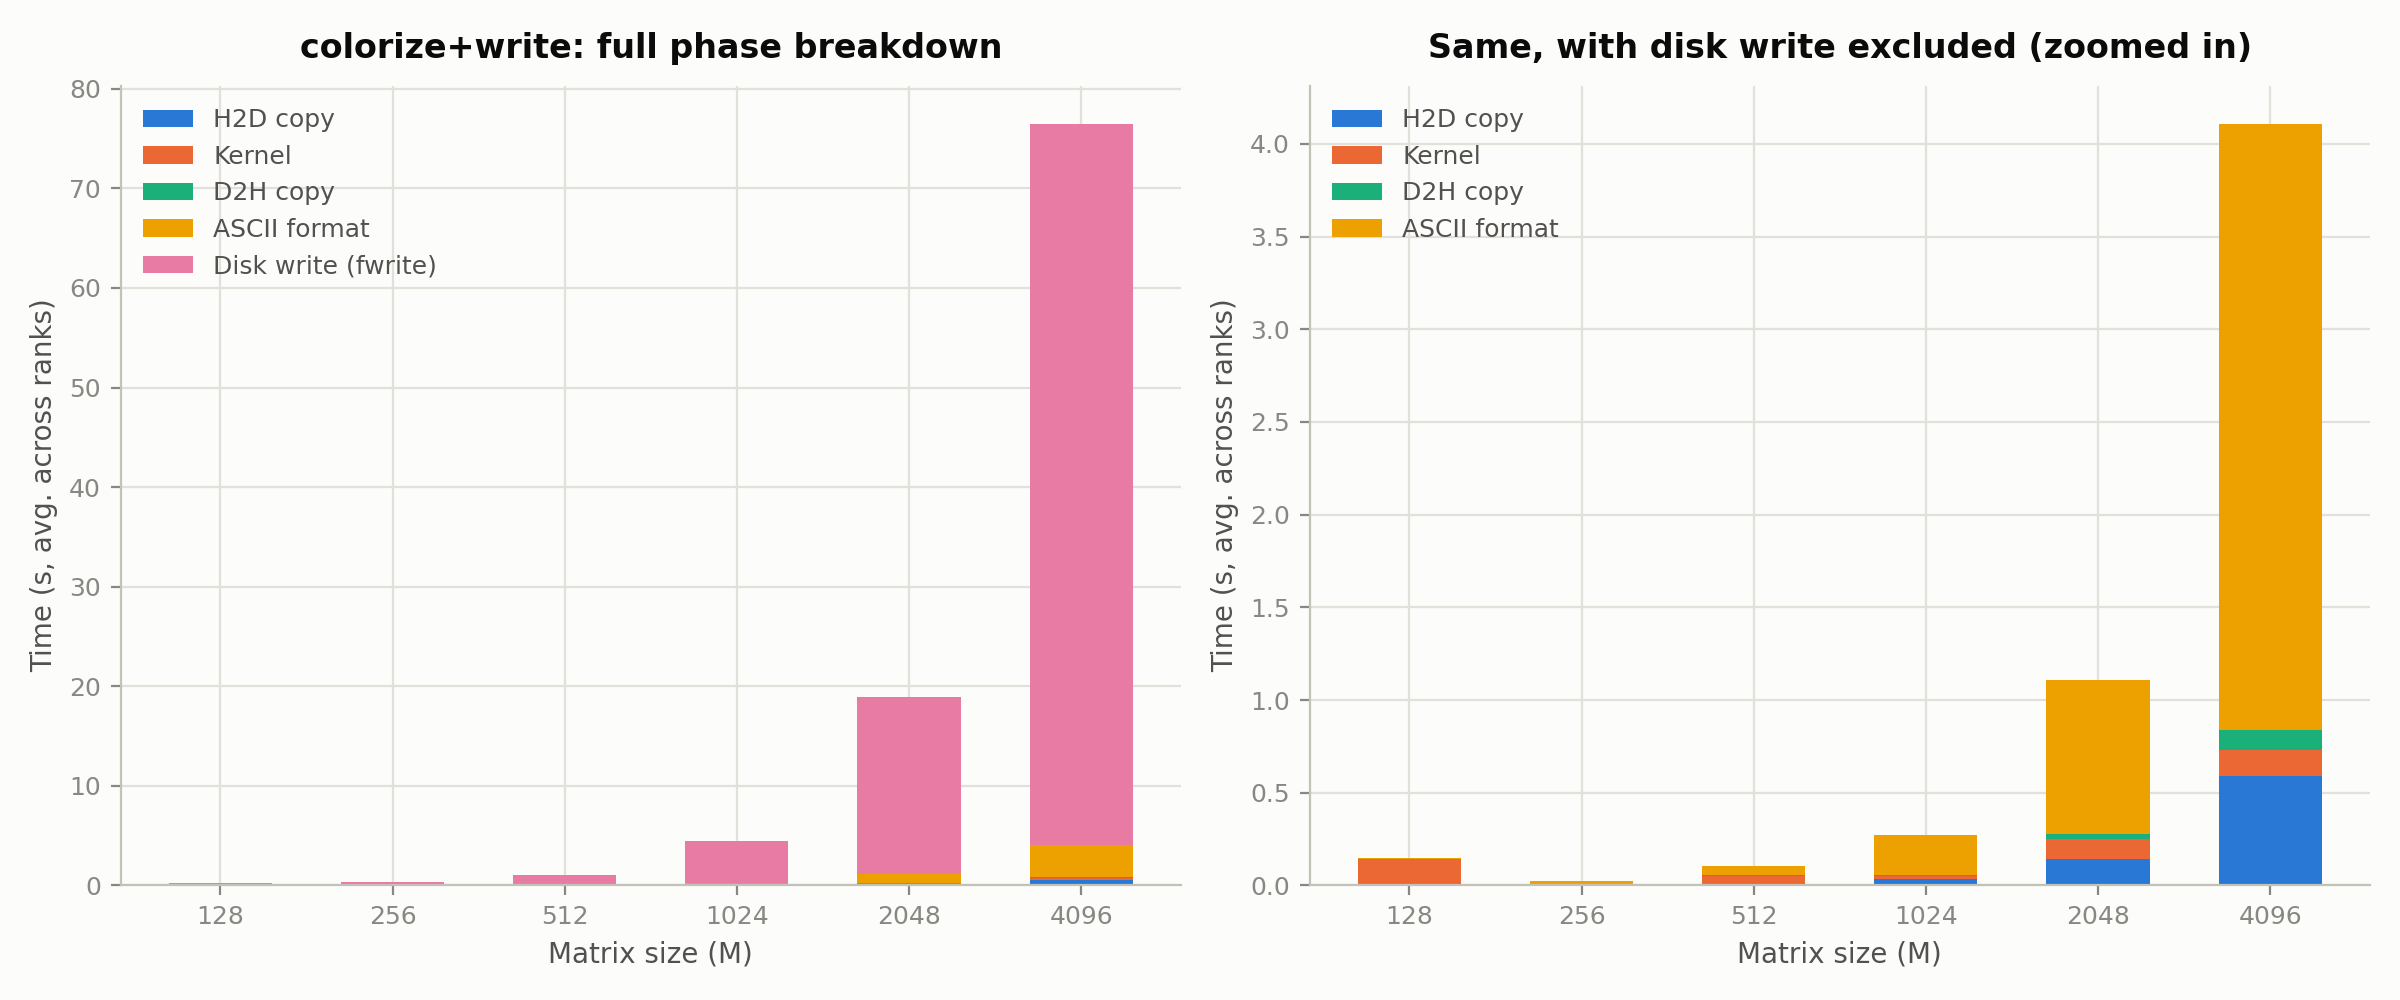
\includegraphics[width=0.68\textwidth]{../src/Davide/Final/Latex/figures/size_sweep_phase_breakdown.png}
    \caption{colorize+write split into its 5 phases vs.\ grid size. Left: full stack (write's dominance is the point, not log-scaled). Right: same data with write excluded, zoomed in.}
    \label{fig:phase}
\end{figure}

\subsection{Where does the write time actually go? Nsight Systems, cross-checked on two GPUs}
\label{sec:nsys}
Nsight Compute (kernel-level occupancy/throughput metrics) was
attempted but is unavailable on this cluster: it returns
\texttt{ERR\_NVGPUCTRPERM} -- GPU performance-counter access is
admin-only, a driver-level restriction no user-side flag can work
around. Nsight Systems was used instead, and it revealed something our
own coarse \texttt{write\_s} timer could not: that timer wraps
\texttt{fopen}+\texttt{fwrite}+\texttt{fclose} as one block, and Nsight
Systems' OS Runtime Summary lets us split it apart. On \texttt{edu\_a40}:
\texttt{fwrite} itself is cheap ($\sim$0.6\% of total OS-runtime time),
while \texttt{fclose} is $\sim$18.3\% -- roughly 30$\times$ more
expensive than the write call it follows. The two largest categories by
far, \texttt{epoll\_wait} ($\sim$52\%) and \texttt{poll} ($\sim$25\%), we
initially guessed reflected ranks idling on MPI's progress engine. A
follow-up run with MPI event tracing enabled rules that out directly:
summed across \texttt{MPI\_Init}, \texttt{MPI\_Finalize}, and the one
real collective (\texttt{MPI\_Allreduce}), application-level MPI time is
$\sim$0.56s per rank -- under 2\% of the combined
\texttt{epoll\_wait}+\texttt{poll} time ($\sim$28.4s). \texttt{MPI\_Allreduce}
itself is 13.7ms. The better-supported explanation, from a companion
VTune Threading run on the same job: its top wait objects include
InfiniBand verbs streams (\texttt{/dev/infiniband/uverbs0}), suggesting
OpenMPI's UCX transport stack is initialized and idly polling in the
background for the whole process lifetime regardless of how little it is
actually used -- not the application's own collective calls, but the
runtime's transport layer underneath them. We report this as the
better-supported hypothesis, not a fully isolated cause. To check whether the OS-runtime pattern itself is an artifact of
one specific GPU, we repeated the identical run on \texttt{edu\_v100} --
an older GPU generation with a slower host interconnect (the whole
production run was $\sim$3$\times$ slower end-to-end on V100, consistent
with H2D transfer time alone rising from $\sim$52\% to $\sim$67\% of GPU
time). Despite the large hardware difference, the OS-runtime split is
nearly identical (Figure~\ref{fig:nsys}): \texttt{fclose} $\sim$17.9\%,
\texttt{fwrite} $\sim$0.4\%, \texttt{epoll\_wait}+\texttt{poll}
$\sim$76\% combined on both. This is good evidence the bottleneck is
I/O/synchronization behavior, not GPU-specific.

\begin{figure}[h]
    \centering
    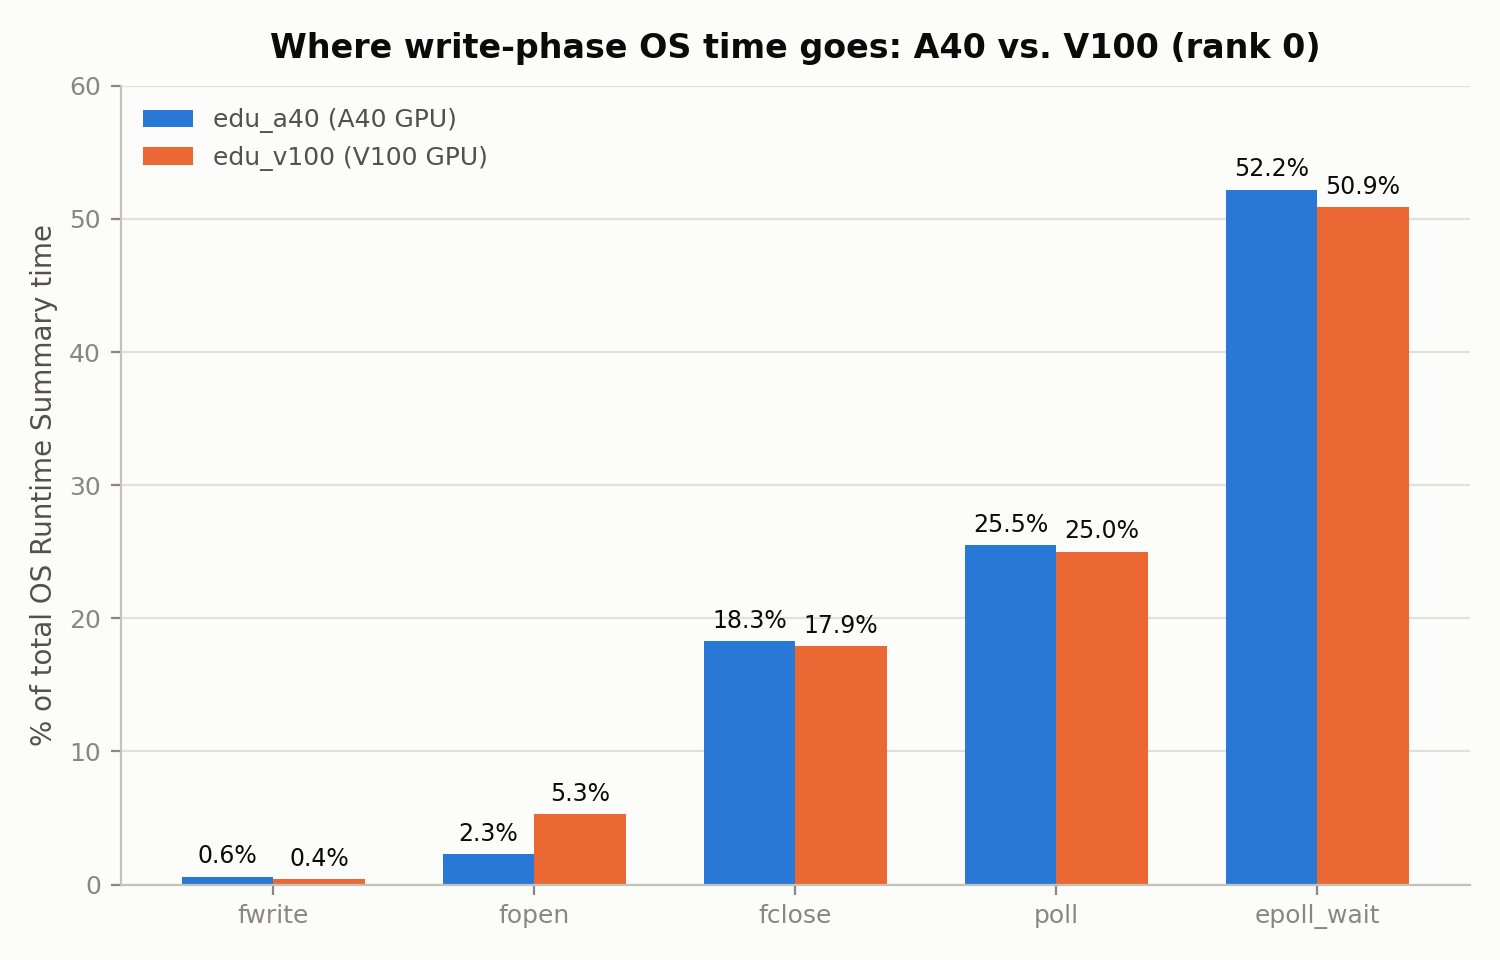
\includegraphics[width=0.6\textwidth]{../src/Davide/Final/Latex/figures/nsys_os_runtime_breakdown.png}
    \caption{OS Runtime Summary breakdown (rank 0), \texttt{edu\_a40} vs.\ \texttt{edu\_v100} -- nearly identical despite very different GPU hardware.}
    \label{fig:nsys}
\end{figure}

\subsection{OpenMP thread scaling and CUDA block size}
Figure~\ref{fig:thread} sweeps OpenMP thread count 1--32 at $M=4096$ (the
full logical-core range of one \texttt{edu\_a40} rank, $96/3$). Both the
full-pipeline and \texttt{compute\_next}-only curves are essentially
flat, never exceeding $\sim$1.2$\times$ speedup, with compute-only
plateauing by 2 threads and staying flat through 32. This is consistent
with the 5-point stencil being memory-bandwidth-bound rather than
compute-bound (4 loads, 1 store, few FLOPs per point) -- a small number
of threads already saturates available memory bandwidth. We also
considered an alternative explanation -- that \texttt{compute\_next}
forking a fresh OpenMP thread team on every one of 300 calls/rank could
plateau this curve through fork/join overhead alone, independent of
memory bandwidth -- and ruled it out with VTune Hotspots at $M=4096$:
\texttt{gomp\_team\_barrier\_wait\_end} does not appear among the top
hotspots at either 4 or 32 threads (unlike part 1's profile, where it was
79.4\% of CPU time), and \texttt{compute\_next}'s own CPU time is flat
across that range (3.43s at 4 threads vs.\ 3.21s at 32) rather than
growing with team size. This contrasts
with part 1's own OpenMP results, which showed real scaling at large
thread counts, mainly because part 1 tested $M$ up to 15000 -- large
enough for the stencil's absolute cost to be interesting on its own,
with no competing GPU-bound stage.

\begin{figure}[h]
    \centering
    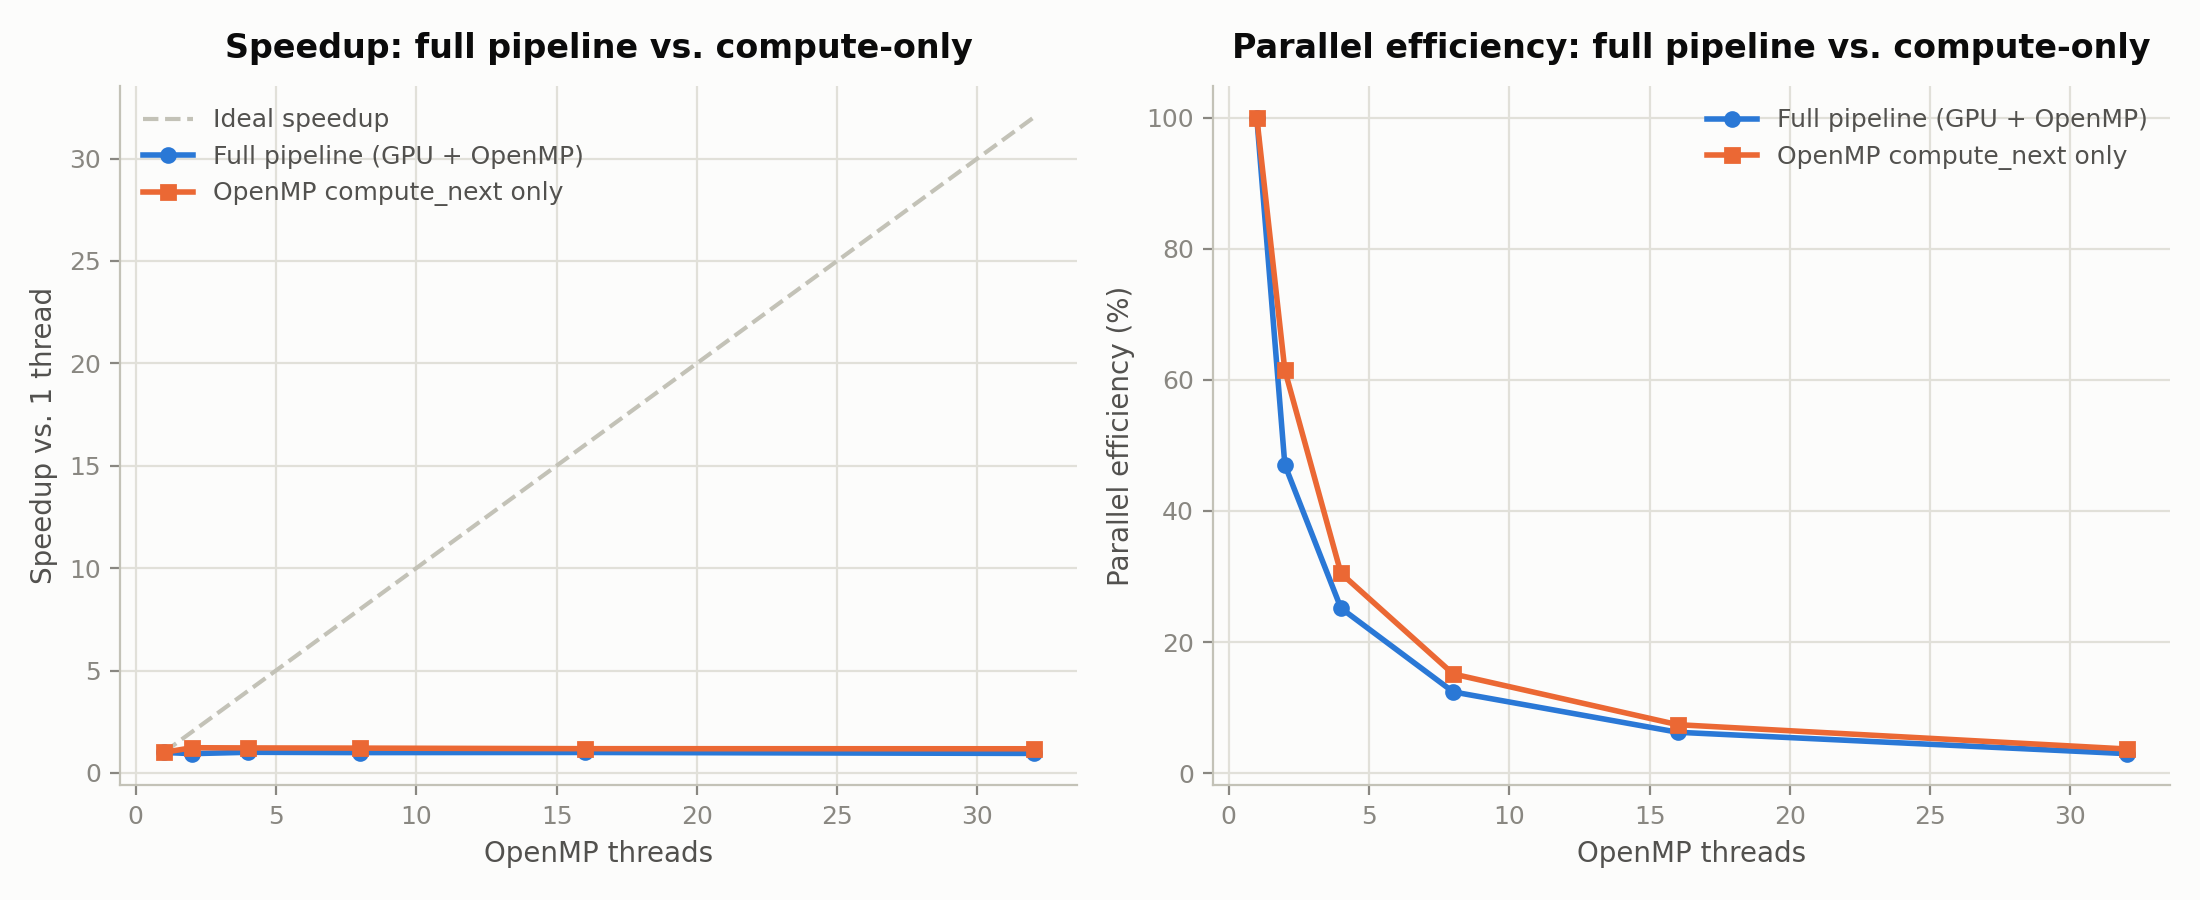
\includegraphics[width=0.68\textwidth]{../src/Davide/Final/Latex/figures/thread_sweep_speedup_efficiency.png}
    \caption{Speedup and efficiency vs.\ OpenMP thread count at $M=4096$, full pipeline vs.\ compute-only.}
    \label{fig:thread}
\end{figure}

Figure~\ref{fig:block} sweeps the CUDA kernel's threads-per-block at
$M=4096$: time decreases roughly monotonically as block size grows,
worst at 32 threads/block ($\sim$83s average) and best at 1024
($\sim$73s, $\sim$12\% faster), with only a minor plateau between 128
and 512. Since Nsight Compute (the tool that would report actual
occupancy) is unavailable on this cluster, we do not have a
profiler-level explanation for this trend, only the timing result
itself -- the most we can say is that fewer, larger blocks amortize
per-block launch and scheduling overhead across more threads. A smaller,
noisier earlier sweep at $M=1024$ (not shown) trended the opposite way
at the high end, so we do not treat this shape as independently
confirmed and report only the $M=4096$ result.

\begin{figure}[h]
    \centering
    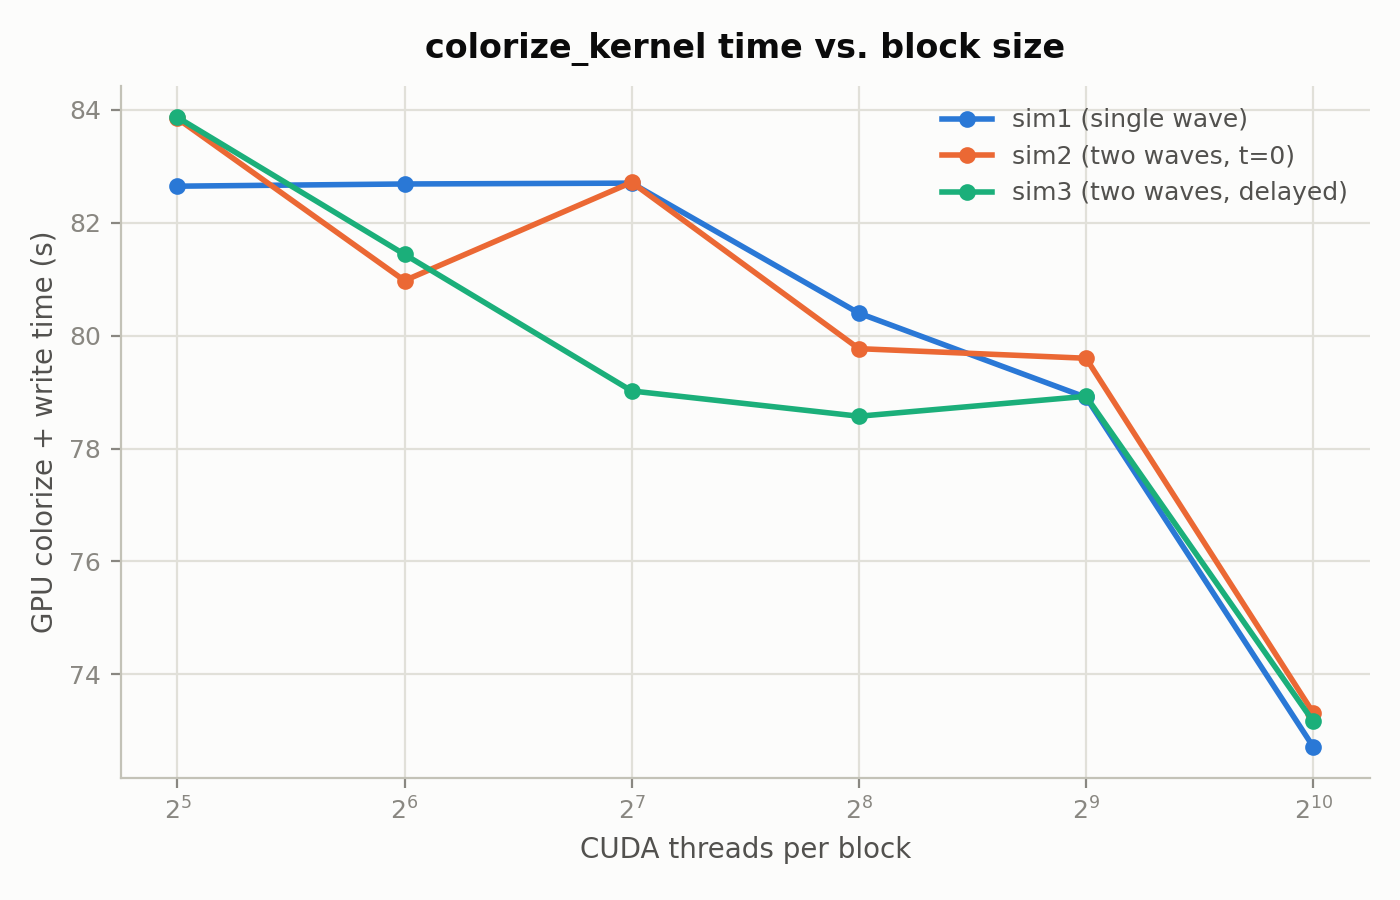
\includegraphics[width=0.52\textwidth]{../src/Davide/Final/Latex/figures/blocksize_sweep_kernel_time.png}
    \caption{GPU colorize+write time vs.\ CUDA threads-per-block, $M=4096$.}
    \label{fig:block}
\end{figure}

\subsection{GPU contention across execution modes}
\label{sec:contention}
Section~\ref{sec:phase} showed disk writes dominate; this raises the
question of how much the design choice of sharing one GPU across 3
ranks actually costs. We compared four execution modes at identical
parameters ($M=2048$, 50 steps, 4 threads), isolating sim1's workload
in each: \texttt{solo} (1 rank, exclusive GPU), \texttt{shared} (the
normal 3-rank/1-GPU run), \texttt{distributed} (3 ranks, 3 dedicated
GPUs on one node, \texttt{--gres=gpu:3}), and \texttt{multinode} (3
ranks on 3 separate nodes, one dedicated GPU each, communicating over
the cluster's Infiniband fabric \cite{sanchezmpitopo}). Results
(Figure~\ref{fig:contention}): \texttt{solo} 9.47s, \texttt{shared}
20.84s, \texttt{distributed} 21.25s, \texttt{multinode} 18.76s.

Two findings. First, dedicating a GPU per rank alone
(\texttt{distributed} vs.\ \texttt{shared}) makes no reliable difference
at all -- \texttt{distributed} is actually $\sim$2\% \emph{slower} here,
well within run-to-run noise rather than a real effect either way --
GPU compute-engine time-slicing is not the bottleneck. Second,
\texttt{solo} is dramatically faster than every multi-rank mode (roughly
half the time, $\sim$50--55\% less depending on which mode it's compared
against), which Section~\ref{sec:phase}'s finding
explains directly: \texttt{shared} and \texttt{distributed} both have 3
ranks writing frames \emph{concurrently} to the same node; \texttt{solo}
is the only mode with exactly one writer at a time, anywhere.
\texttt{multinode} sits in between ($\sim$10\% faster than
\texttt{distributed}) by removing host-local contention (memory bus,
PCIe root complex) but not, most plausibly, a deeper one: all three
nodes most likely still write to the same shared, network-attached
storage behind every node's home directory (per the cluster's own
documentation, though not measured directly here) -- the best available
explanation for why multinode sits closer to \texttt{shared} than to
\texttt{solo}. The dominant contention in this workload is concurrent
I/O, not GPU compute-engine sharing -- consistent with
Section~\ref{sec:nsys}'s \texttt{fclose}-dominated OS Runtime profile.

\begin{figure}[h]
    \centering
    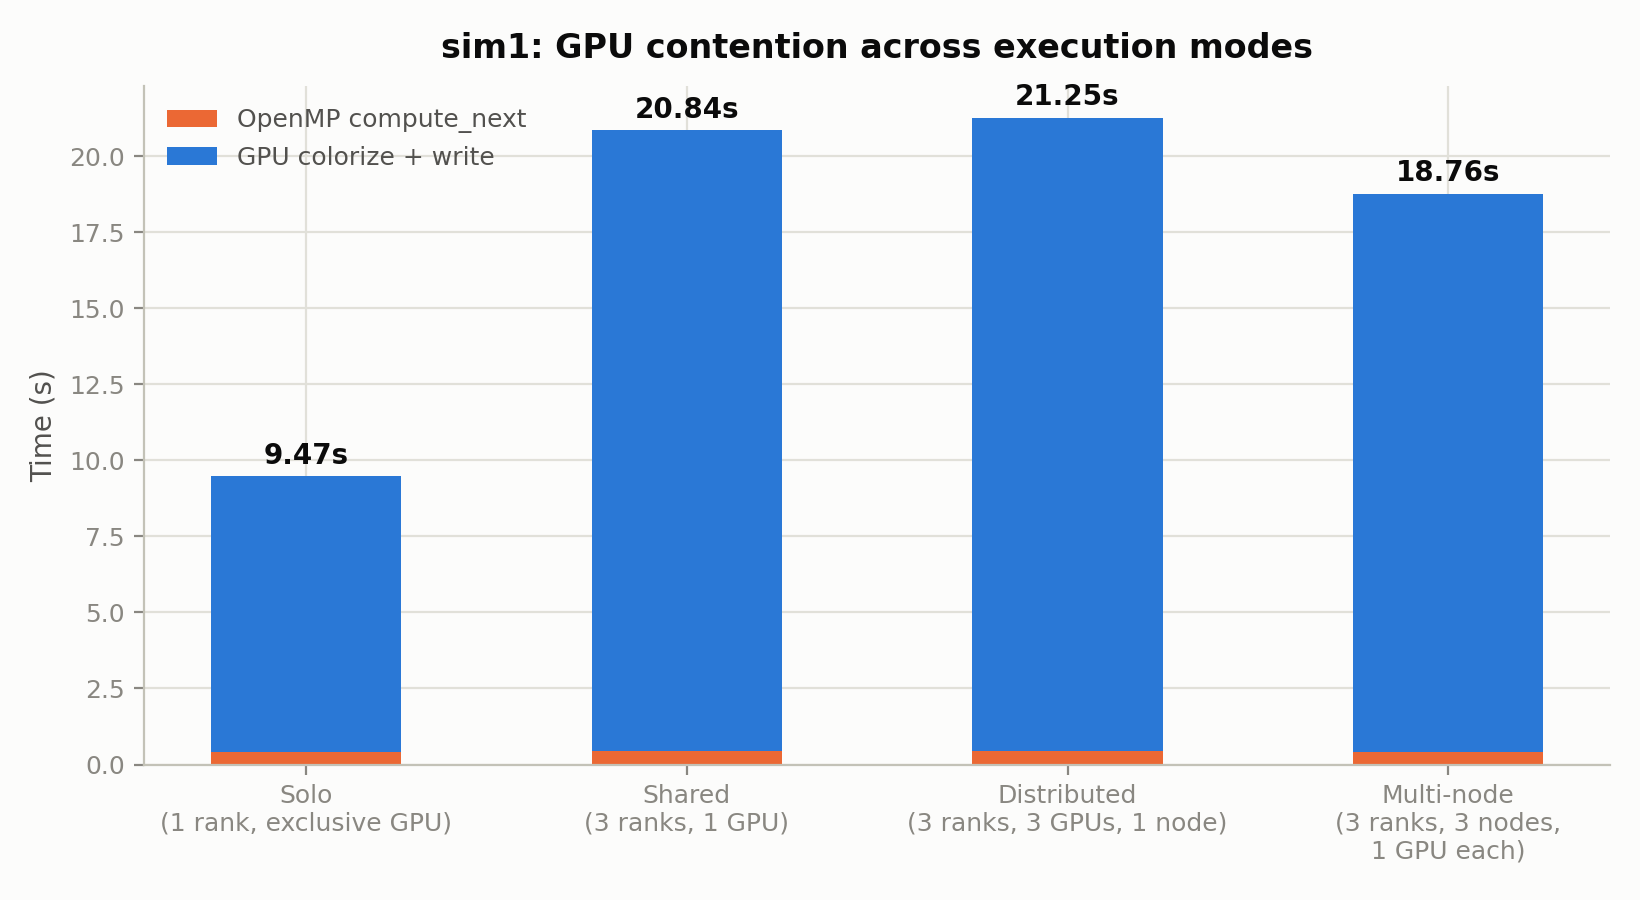
\includegraphics[width=0.6\textwidth]{../src/Davide/Final/Latex/figures/contention_sweep_solo_vs_shared.png}
    \caption{sim1's execution time across four GPU/node sharing configurations, identical workload.}
    \label{fig:contention}
\end{figure}

\subsection{Conclusions}
The dominant cost in this pipeline is not GPU compute (colorization
kernel: $\sim$1\% of frame time) nor CPU compute
(\texttt{compute\_next}: $\sim$2\%), but per-frame file I/O, specifically
whatever happens at \texttt{fclose} time rather than the write itself --
confirmed consistent across two GPU generations and reflected directly
in the GPU-sharing contention results: sharing the GPU across ranks
costs almost nothing, while sharing the filesystem costs a great deal.
This is the throughline of the whole investigation -- every optimization
decision was made only after measuring, not assumed from the physics
alone. Parallelizing the ASCII-formatting step was considered and
rejected once the phase breakdown showed it was $\sim$4\% of
\texttt{color\_time}, not worth the added complexity. Per-frame adaptive
color scaling was adopted only after raw pixel data confirmed a fixed
scale reads as pale almost immediately, since a 2D wave's peak amplitude
falls off geometrically with distance from the source on top of
$\gamma$-damping. And the GPU-sharing question itself was settled by
directly comparing four execution modes rather than assumed from GPU
specifications -- the result (I/O-bound, not compute-bound) held
consistently across every measurement in this report.

% -- report.tex already has graphicx/float in its preamble, and a shared
% report/b.bib for \cite{} (matching assignment_1's convention). All
% \includegraphics paths below are relative to report/, same as
% assignment_1/ass1.tex's own figures.

\section{Assignment 3}

\subsection{Introduction}
This assignment extends the damped wave simulator from parts 1--2 with
color. The physics, discretisation, and MPI/OpenMP structure are
unchanged: three MPI ranks each run one independent scenario (a single
impulse; two impulses starting together; two impulses with the second
delayed to $N/7$), each parallelised with OpenMP. What changes is the
output stage: each timestep's matrix is sent to the GPU, mapped to an RGB
triplet per pixel by a CUDA kernel, and saved as a P3 (ASCII) PPM frame
instead of a grayscale PGM. Bright, saturated colors mark the wave's
extrema, colors fade along the rising/falling fronts, and calm (near-zero)
regions are rendered white. 

%Student parameters (352165): $\gamma=0.067$,
%$c=0.59$, primary impulse at $(M/2,M/2)$ with amplitude 56; sim2's second
%wave at $(2M/3,M/4)$, amplitude $-35$, $t_{\mathrm{start}}=0$; sim3's second
%wave at $(M/3,M/3)$, amplitude 58, $t_{\mathrm{start}}=N/7$.
\subsection{Architecture}
The three MPI
ranks \cite{sanchezmpiintro} map naturally onto the three required
scenarios: each rank owns a complete, independent grid and runs one
scenario end to end, so the only collective call needed is a final
\texttt{MPI\_Allreduce} on success/failure. Within each rank, \texttt{compute\_next}
(the same 5-point Laplacian stencil as parts 1--2 -- each point's next
value is computed from itself and its 4 orthogonal neighbors via central
differences) is parallelised with OpenMP \cite{slidestatic}, using
\texttt{schedule(static)} for the same NUMA first-touch reason argued in
part 1: with a fixed thread-to-row mapping, the memory each thread first
writes (and therefore where the OS physically places it) matches the
memory that same thread repeatedly accesses on every subsequent call. After each timestep, the rank sends its
matrix to the GPU \cite{sanchezcuda}: a kernel normalizes each value
against the frame's own peak magnitude (found via a GPU-side reduction
\cite{sanchezgpuintro}), maps it to a color (white near zero, fading to
bright red/orange for positive values and blue for negative, saturating
at the wave's extrema), and the result is written to disk as an ASCII
PPM frame while the original scalar matrix continues to drive the
simulation.
Because the job requests a single GPU (\texttt{--gres=gpu:1}) for all
three ranks, the GPU is a shared resource -- a design point this report
returns to in Section~\ref{sec:contention}.

\subsection{Cluster hardware}
All experiments ran on Politecnico di Torino's HPC@PoliTO cluster
(Legion), specifically its EDU partitions -- reserved for coursework,
as opposed to the open-access or research-group-restricted partitions
also present on the cluster. Of the four EDU partitions, only two have
GPUs: \texttt{edu\_a40} and \texttt{edu\_v100}, confirmed live via
\texttt{sinfo -o "\%P \%D \%G"} (the other two, \texttt{edu\_skylake}
and \texttt{edu\_sapphire}, are CPU-only). \texttt{edu\_a40} nodes have 2 physical CPU sockets, 24 physical cores
per socket (48 physical cores/node), doubled to 96 logical cores/node by
SMT (2 hardware threads per core) -- confirmed via \texttt{sinfo}'s
socket/core/thread fields, since the cluster's own documentation lists
only the 48 physical cores -- and 4$\times$A40 GPUs;
\texttt{edu\_v100} nodes have 32 cores and 4$\times$V100 GPUs. Both are
used in this report: \texttt{edu\_a40} for all main results, and
\texttt{edu\_v100} as a cross-hardware check in Section~\ref{sec:nsys}.

\subsection{Metrics and the grid-size sweep}
\label{sec:metrics}
Beyond wall-clock time, the program times two phases directly:
\texttt{color\_time} (GPU colorization + PPM write, per frame) and
\texttt{compute\_time} (the OpenMP stencil update). \texttt{color\_time}
is further split into five sub-phases -- H2D copy, kernel, D2H copy,
ASCII formatting, and disk write -- introduced in
Section~\ref{sec:phase}. Figure~\ref{fig:size} sweeps grid size $M$ from
128 to 4096 (\texttt{edu\_a40}, 4 threads, 50 steps). Execution time
approaches ideal $O(M^2)$ scaling as $M$ grows: $128\to256$ costs only
$2.1\times$ (fixed per-run overhead still dominant at small $M$), while
$2048\to4096$ costs $4.1\times$ -- essentially the ideal quadratic ratio.
The right panel shows GPU colorize+write dominating total time
throughout: at $M=4096$ it is $\sim$97.6\% of total time, versus
\texttt{compute\_next} at $\sim$2.4\%. Both phases are $O(M^2)$, so this
ratio stays roughly constant across the whole sweep ($\sim$97.6--97.7\%
from $M=256$ upward; only the smallest grid, $M=128$, deviates, where
fixed per-run overhead is large enough to matter).

We capped the sweep at $M=4096$ rather than matching part 1's $M=15000$:
at $M=4096$ an ASCII PPM frame is already $\sim$100--130MB, so scaling to
$M=15000$ -- $(15000/4096)^2\approx13\times$ the pixels -- would push
single frames into the multi-gigabyte range across 50 steps and 3 ranks,
for a sweep whose purpose (showing execution time approach ideal
$O(M^2)$ scaling and locating the point where GPU colorize+write comes
to dominate) was already unambiguous well before $M=4096$.

\begin{figure}[h]
    \centering
    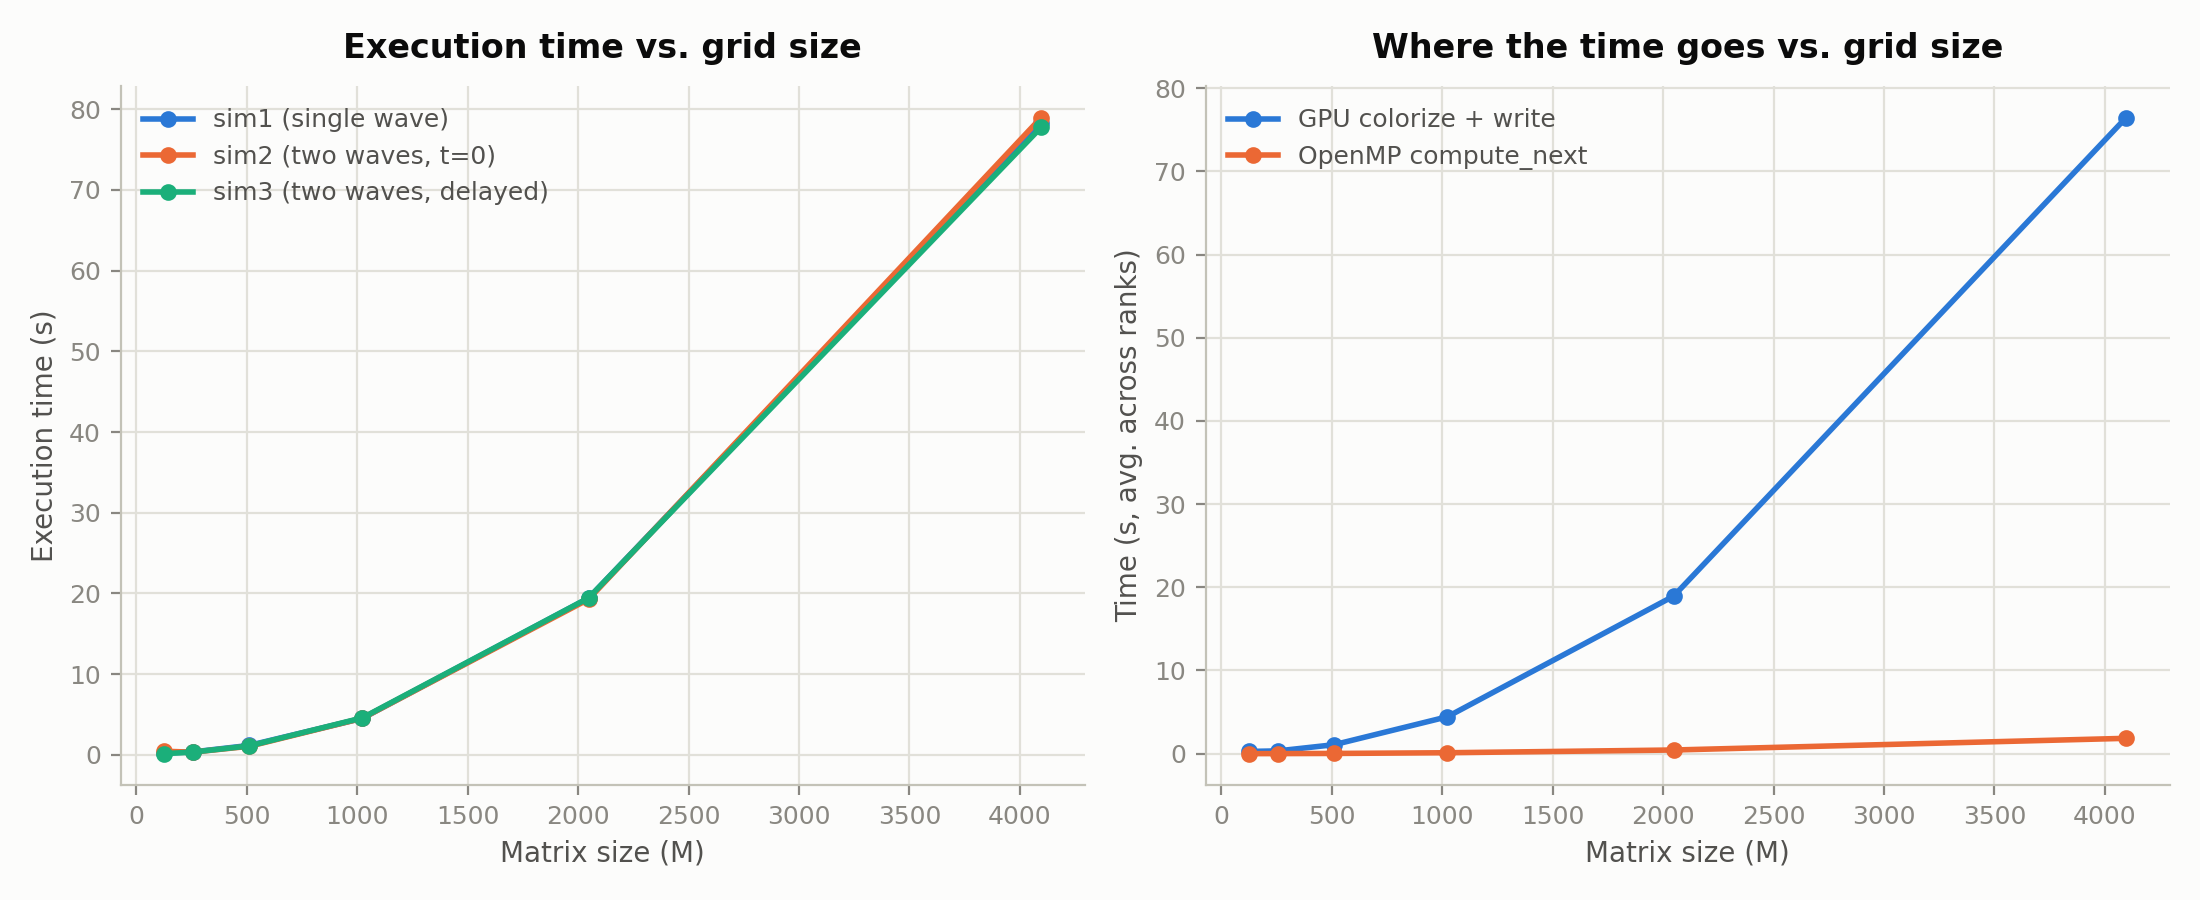
\includegraphics[width=0.68\textwidth]{../src/Davide/Final/Latex/figures/size_sweep_execution_time.png}
    \caption{Execution time and its GPU/OpenMP split, varying grid size $M$ (4 threads, 3 ranks sharing 1 GPU).}
    \label{fig:size}
\end{figure}

\subsection{Phase breakdown: is the ASCII formatting worth parallelizing?}
\label{sec:phase}
Figure~\ref{fig:phase} breaks \texttt{color\_time} into its five
sub-phases. At $M=4096$ (averaged over 3 ranks): \texttt{write} (the
\texttt{fwrite} call) is $\sim$94.6\% of \texttt{color\_time},
\texttt{format} (the ASCII byte-to-digit conversion) is $\sim$4.3\%, and
H2D copy + kernel + D2H copy combined are $\sim$1\%. The same lopsided
pattern holds at every grid size swept, not only at $M=4096$.

This directly answers a question we considered early on: is it worth
parallelizing the ASCII-formatting step with OpenMP? It is not --
formatting is only $\sim$4\% of \texttt{color\_time}, so even a
theoretical zero-overhead parallelization would save a few percent of
total time at best, not worth the added complexity (the output is
variable-width per pixel, so parallel writers would need either a
prefix-sum pass to compute offsets first, or a switch to fixed-width
padding). We measured before optimizing, and the measurement said no.

\begin{figure}[h]
    \centering
    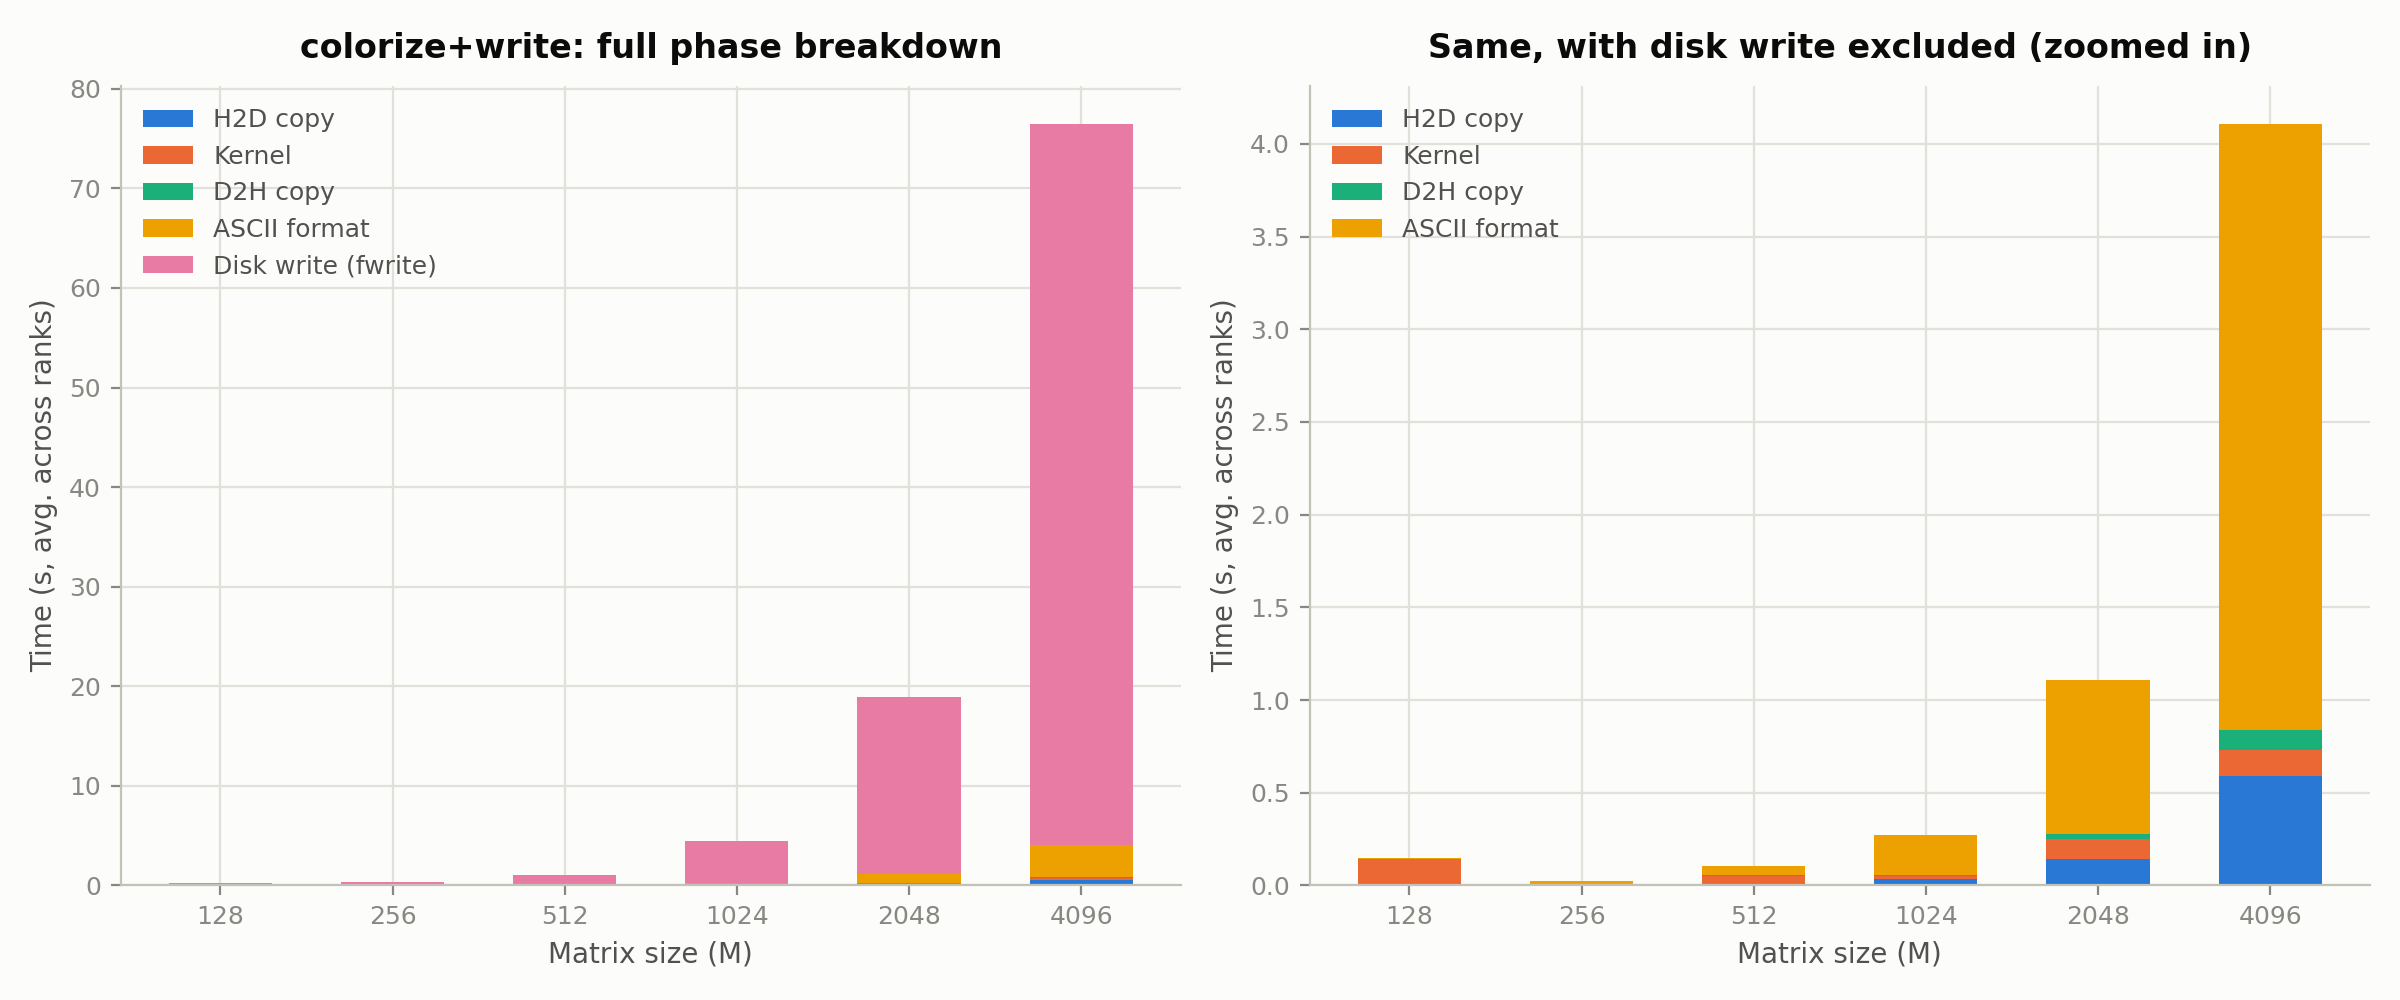
\includegraphics[width=0.68\textwidth]{../src/Davide/Final/Latex/figures/size_sweep_phase_breakdown.png}
    \caption{colorize+write split into its 5 phases vs.\ grid size. Left: full stack (write's dominance is the point, not log-scaled). Right: same data with write excluded, zoomed in.}
    \label{fig:phase}
\end{figure}

\subsection{Where does the write time actually go? Nsight Systems, cross-checked on two GPUs}
\label{sec:nsys}
Nsight Compute (kernel-level occupancy/throughput metrics) was
attempted but is unavailable on this cluster: it returns
\texttt{ERR\_NVGPUCTRPERM} -- GPU performance-counter access is
admin-only, a driver-level restriction no user-side flag can work
around. Nsight Systems was used instead, and it revealed something our
own coarse \texttt{write\_s} timer could not: that timer wraps
\texttt{fopen}+\texttt{fwrite}+\texttt{fclose} as one block, and Nsight
Systems' OS Runtime Summary lets us split it apart. On \texttt{edu\_a40}:
\texttt{fwrite} itself is cheap ($\sim$0.6\% of total OS-runtime time),
while \texttt{fclose} is $\sim$18.3\% -- roughly 30$\times$ more
expensive than the write call it follows. The two largest categories by
far, \texttt{epoll\_wait} ($\sim$52\%) and \texttt{poll} ($\sim$25\%), we
initially guessed reflected ranks idling on MPI's progress engine. A
follow-up run with MPI event tracing enabled rules that out directly:
summed across \texttt{MPI\_Init}, \texttt{MPI\_Finalize}, and the one
real collective (\texttt{MPI\_Allreduce}), application-level MPI time is
$\sim$0.56s per rank -- under 2\% of the combined
\texttt{epoll\_wait}+\texttt{poll} time ($\sim$28.4s). \texttt{MPI\_Allreduce}
itself is 13.7ms. The better-supported explanation, from a companion
VTune Threading run on the same job: its top wait objects include
InfiniBand verbs streams (\texttt{/dev/infiniband/uverbs0}), suggesting
OpenMPI's UCX transport stack is initialized and idly polling in the
background for the whole process lifetime regardless of how little it is
actually used -- not the application's own collective calls, but the
runtime's transport layer underneath them. We report this as the
better-supported hypothesis, not a fully isolated cause. To check whether the OS-runtime pattern itself is an artifact of
one specific GPU, we repeated the identical run on \texttt{edu\_v100} --
an older GPU generation with a slower host interconnect (the whole
production run was $\sim$3$\times$ slower end-to-end on V100, consistent
with H2D transfer time alone rising from $\sim$52\% to $\sim$67\% of GPU
time). Despite the large hardware difference, the OS-runtime split is
nearly identical (Figure~\ref{fig:nsys}): \texttt{fclose} $\sim$17.9\%,
\texttt{fwrite} $\sim$0.4\%, \texttt{epoll\_wait}+\texttt{poll}
$\sim$76\% combined on both. This is good evidence the bottleneck is
I/O/synchronization behavior, not GPU-specific.

\begin{figure}[h]
    \centering
    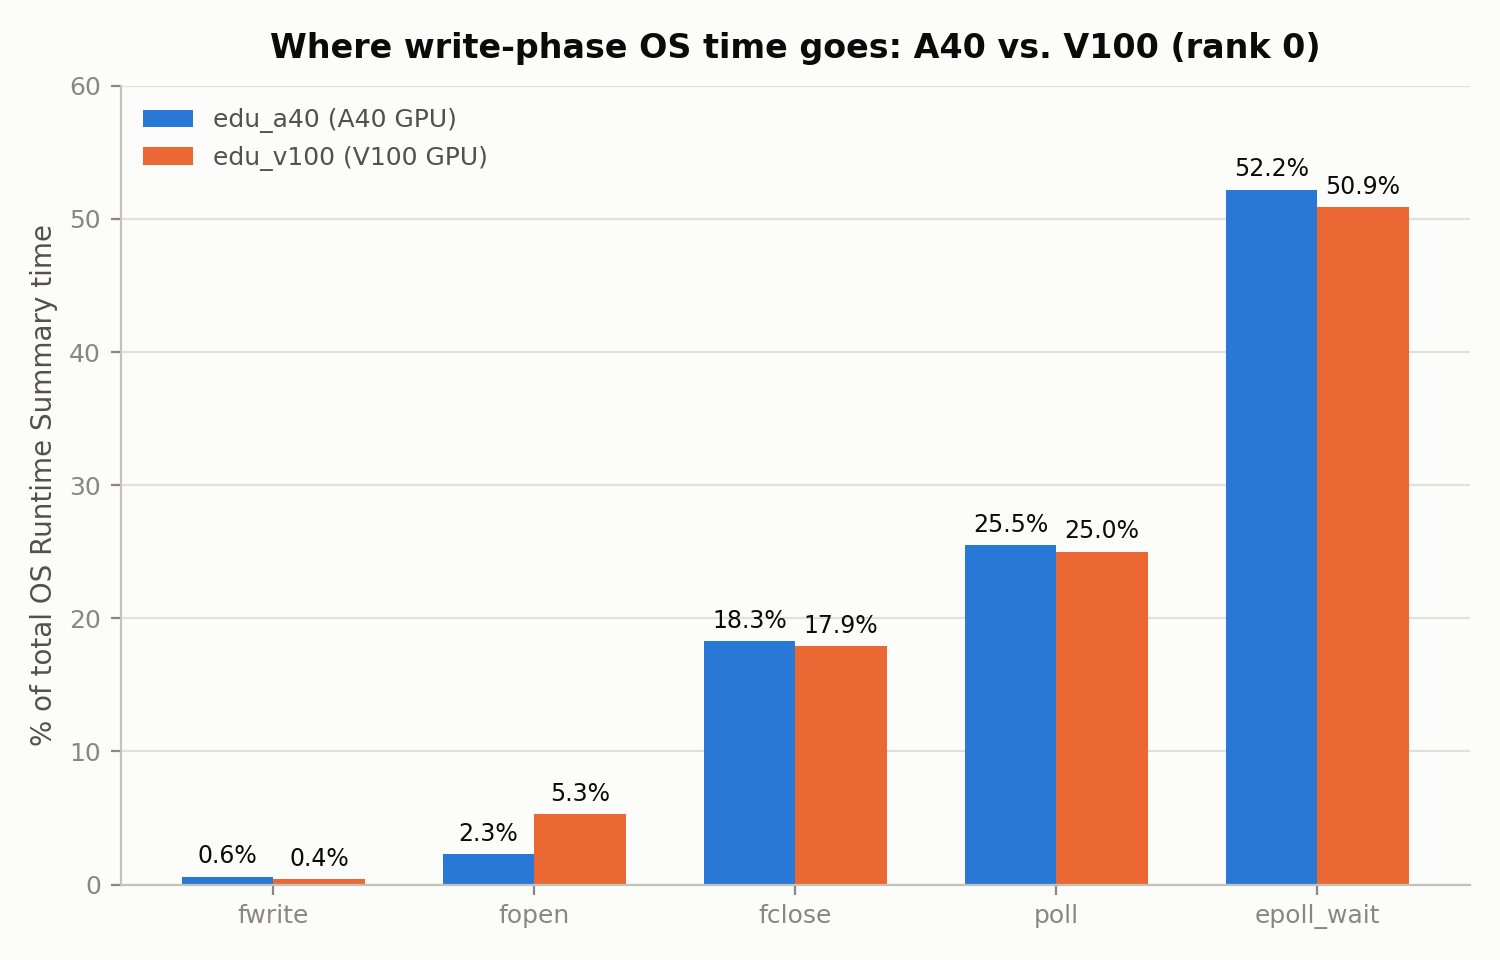
\includegraphics[width=0.6\textwidth]{../src/Davide/Final/Latex/figures/nsys_os_runtime_breakdown.png}
    \caption{OS Runtime Summary breakdown (rank 0), \texttt{edu\_a40} vs.\ \texttt{edu\_v100} -- nearly identical despite very different GPU hardware.}
    \label{fig:nsys}
\end{figure}

\subsection{OpenMP thread scaling and CUDA block size}
Figure~\ref{fig:thread} sweeps OpenMP thread count 1--32 at $M=4096$ (the
full logical-core range of one \texttt{edu\_a40} rank, $96/3$). Both the
full-pipeline and \texttt{compute\_next}-only curves are essentially
flat, never exceeding $\sim$1.2$\times$ speedup, with compute-only
plateauing by 2 threads and staying flat through 32. This is consistent
with the 5-point stencil being memory-bandwidth-bound rather than
compute-bound (4 loads, 1 store, few FLOPs per point) -- a small number
of threads already saturates available memory bandwidth. We also
considered an alternative explanation -- that \texttt{compute\_next}
forking a fresh OpenMP thread team on every one of 300 calls/rank could
plateau this curve through fork/join overhead alone, independent of
memory bandwidth -- and ruled it out with VTune Hotspots at $M=4096$:
\texttt{gomp\_team\_barrier\_wait\_end} does not appear among the top
hotspots at either 4 or 32 threads (unlike part 1's profile, where it was
79.4\% of CPU time), and \texttt{compute\_next}'s own CPU time is flat
across that range (3.43s at 4 threads vs.\ 3.21s at 32) rather than
growing with team size. This contrasts
with part 1's own OpenMP results, which showed real scaling at large
thread counts, mainly because part 1 tested $M$ up to 15000 -- large
enough for the stencil's absolute cost to be interesting on its own,
with no competing GPU-bound stage.

\begin{figure}[h]
    \centering
    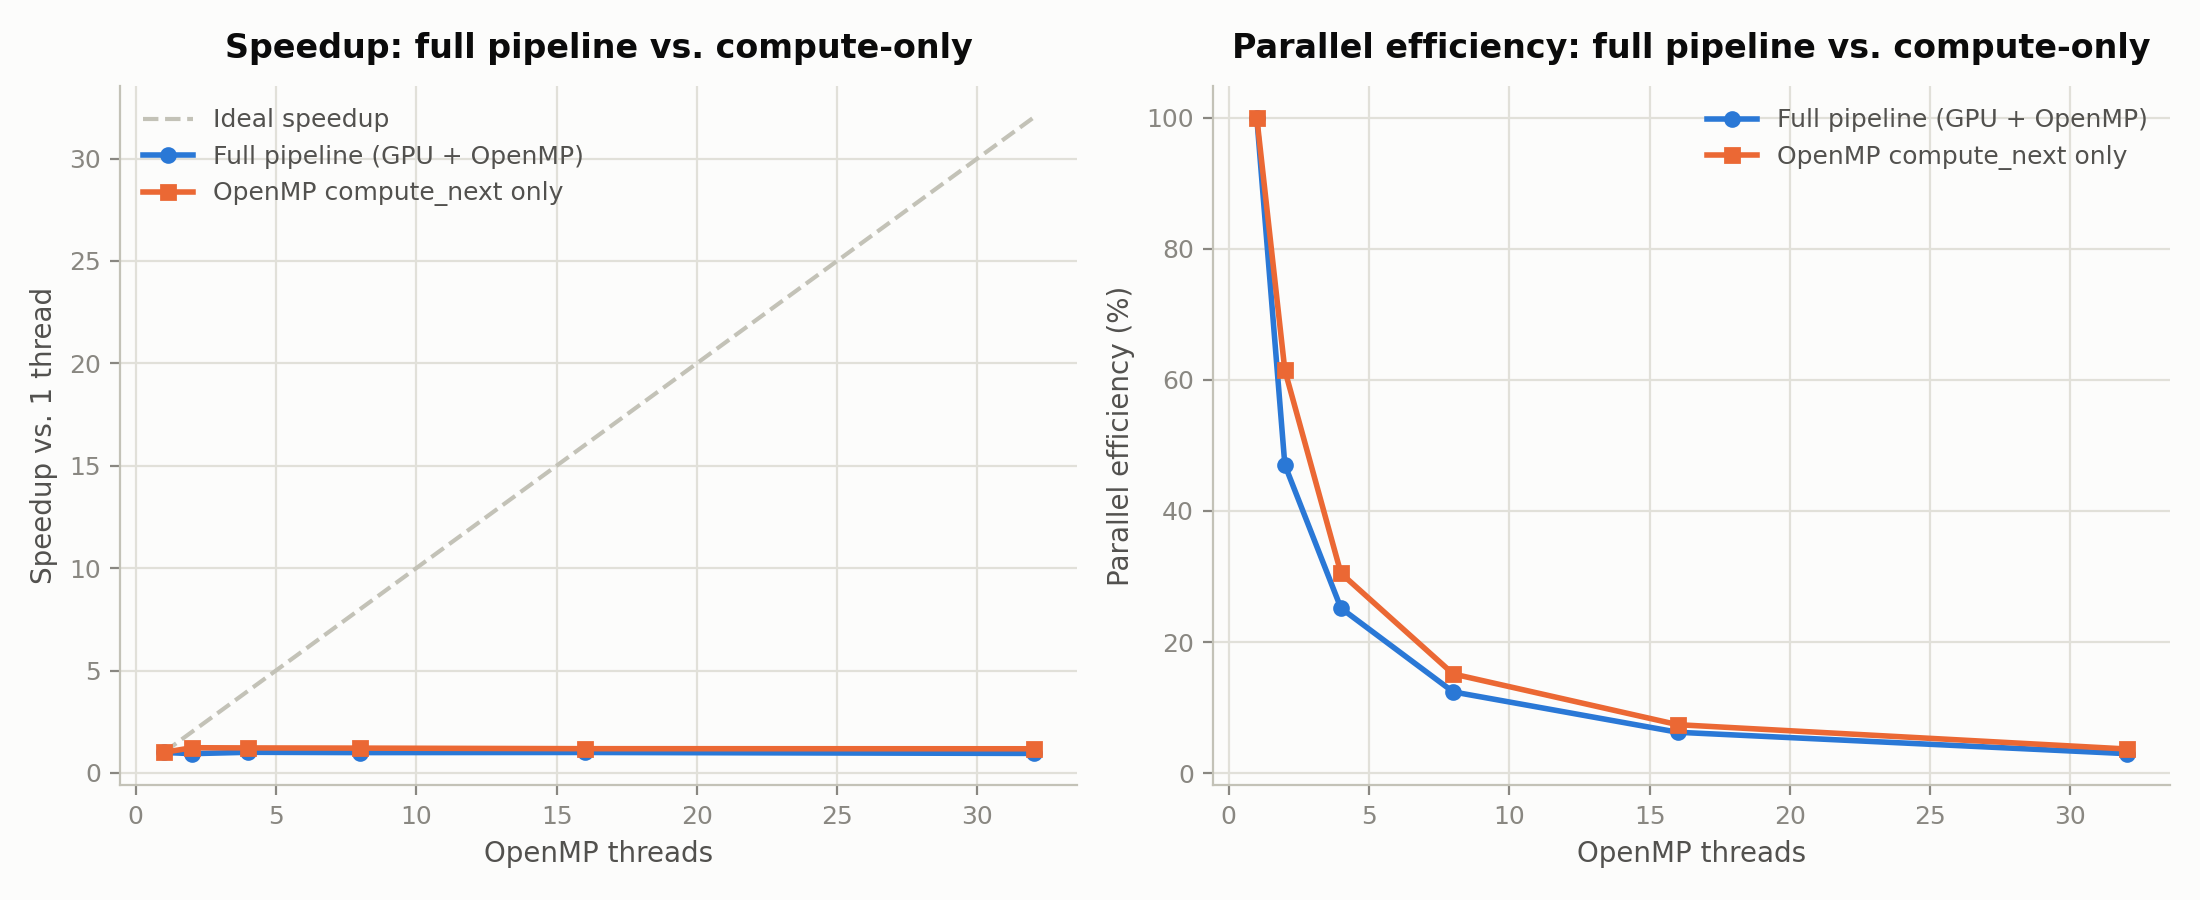
\includegraphics[width=0.68\textwidth]{../src/Davide/Final/Latex/figures/thread_sweep_speedup_efficiency.png}
    \caption{Speedup and efficiency vs.\ OpenMP thread count at $M=4096$, full pipeline vs.\ compute-only.}
    \label{fig:thread}
\end{figure}

Figure~\ref{fig:block} sweeps the CUDA kernel's threads-per-block at
$M=4096$: time decreases roughly monotonically as block size grows,
worst at 32 threads/block ($\sim$83s average) and best at 1024
($\sim$73s, $\sim$12\% faster), with only a minor plateau between 128
and 512. Since Nsight Compute (the tool that would report actual
occupancy) is unavailable on this cluster, we do not have a
profiler-level explanation for this trend, only the timing result
itself -- the most we can say is that fewer, larger blocks amortize
per-block launch and scheduling overhead across more threads. A smaller,
noisier earlier sweep at $M=1024$ (not shown) trended the opposite way
at the high end, so we do not treat this shape as independently
confirmed and report only the $M=4096$ result.

\begin{figure}[h]
    \centering
    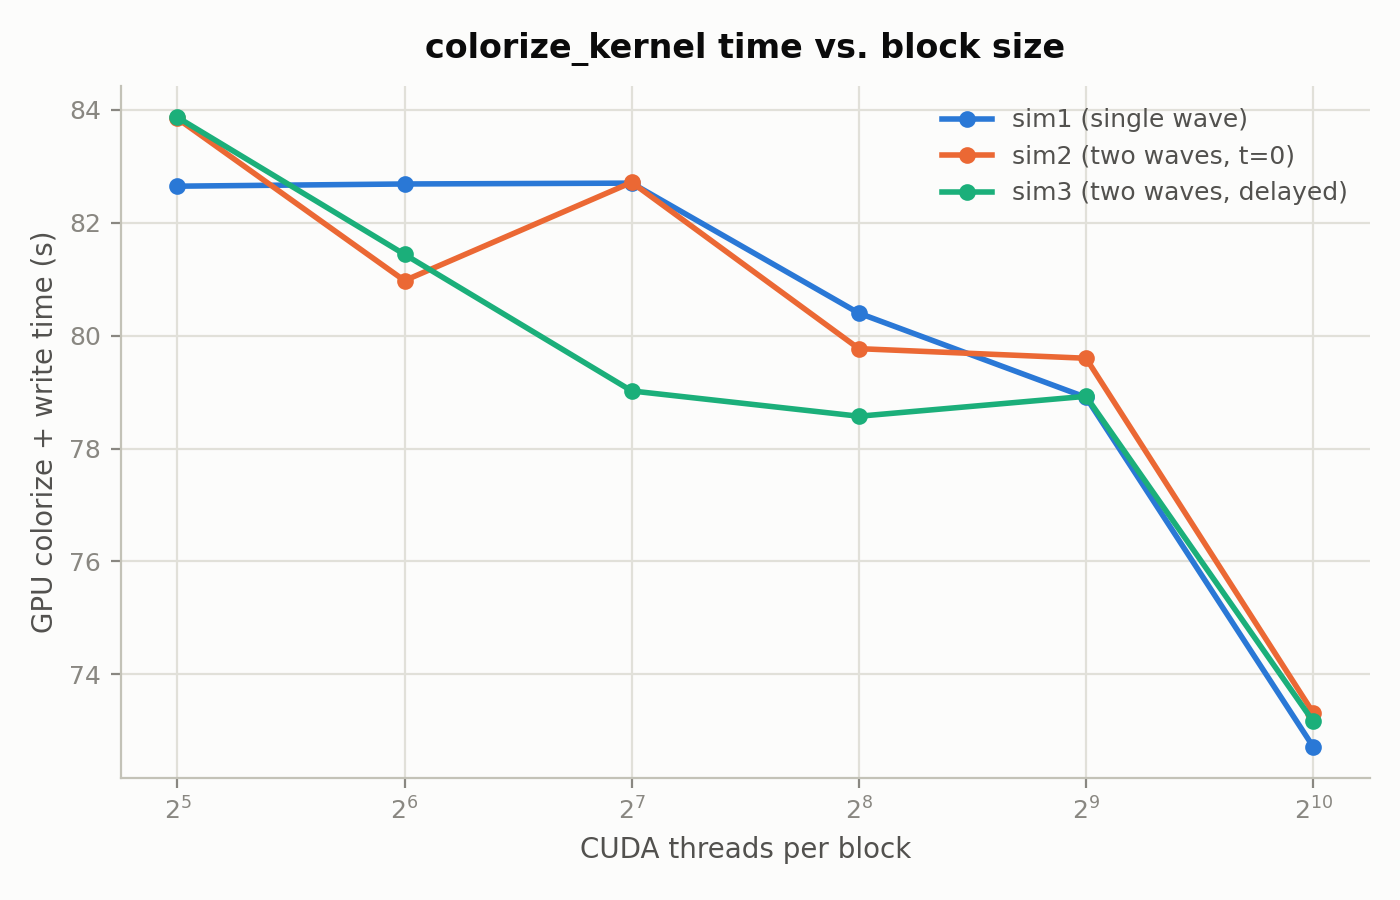
\includegraphics[width=0.52\textwidth]{../src/Davide/Final/Latex/figures/blocksize_sweep_kernel_time.png}
    \caption{GPU colorize+write time vs.\ CUDA threads-per-block, $M=4096$.}
    \label{fig:block}
\end{figure}

\subsection{GPU contention across execution modes}
\label{sec:contention}
Section~\ref{sec:phase} showed disk writes dominate; this raises the
question of how much the design choice of sharing one GPU across 3
ranks actually costs. We compared four execution modes at identical
parameters ($M=2048$, 50 steps, 4 threads), isolating sim1's workload
in each: \texttt{solo} (1 rank, exclusive GPU), \texttt{shared} (the
normal 3-rank/1-GPU run), \texttt{distributed} (3 ranks, 3 dedicated
GPUs on one node, \texttt{--gres=gpu:3}), and \texttt{multinode} (3
ranks on 3 separate nodes, one dedicated GPU each, communicating over
the cluster's Infiniband fabric \cite{sanchezmpitopo}). Results
(Figure~\ref{fig:contention}): \texttt{solo} 9.47s, \texttt{shared}
20.84s, \texttt{distributed} 21.25s, \texttt{multinode} 18.76s.

Two findings. First, dedicating a GPU per rank alone
(\texttt{distributed} vs.\ \texttt{shared}) makes no reliable difference
at all -- \texttt{distributed} is actually $\sim$2\% \emph{slower} here,
well within run-to-run noise rather than a real effect either way --
GPU compute-engine time-slicing is not the bottleneck. Second,
\texttt{solo} is dramatically faster than every multi-rank mode (roughly
half the time, $\sim$50--55\% less depending on which mode it's compared
against), which Section~\ref{sec:phase}'s finding
explains directly: \texttt{shared} and \texttt{distributed} both have 3
ranks writing frames \emph{concurrently} to the same node; \texttt{solo}
is the only mode with exactly one writer at a time, anywhere.
\texttt{multinode} sits in between ($\sim$10\% faster than
\texttt{distributed}) by removing host-local contention (memory bus,
PCIe root complex) but not, most plausibly, a deeper one: all three
nodes most likely still write to the same shared, network-attached
storage behind every node's home directory (per the cluster's own
documentation, though not measured directly here) -- the best available
explanation for why multinode sits closer to \texttt{shared} than to
\texttt{solo}. The dominant contention in this workload is concurrent
I/O, not GPU compute-engine sharing -- consistent with
Section~\ref{sec:nsys}'s \texttt{fclose}-dominated OS Runtime profile.

\begin{figure}[h]
    \centering
    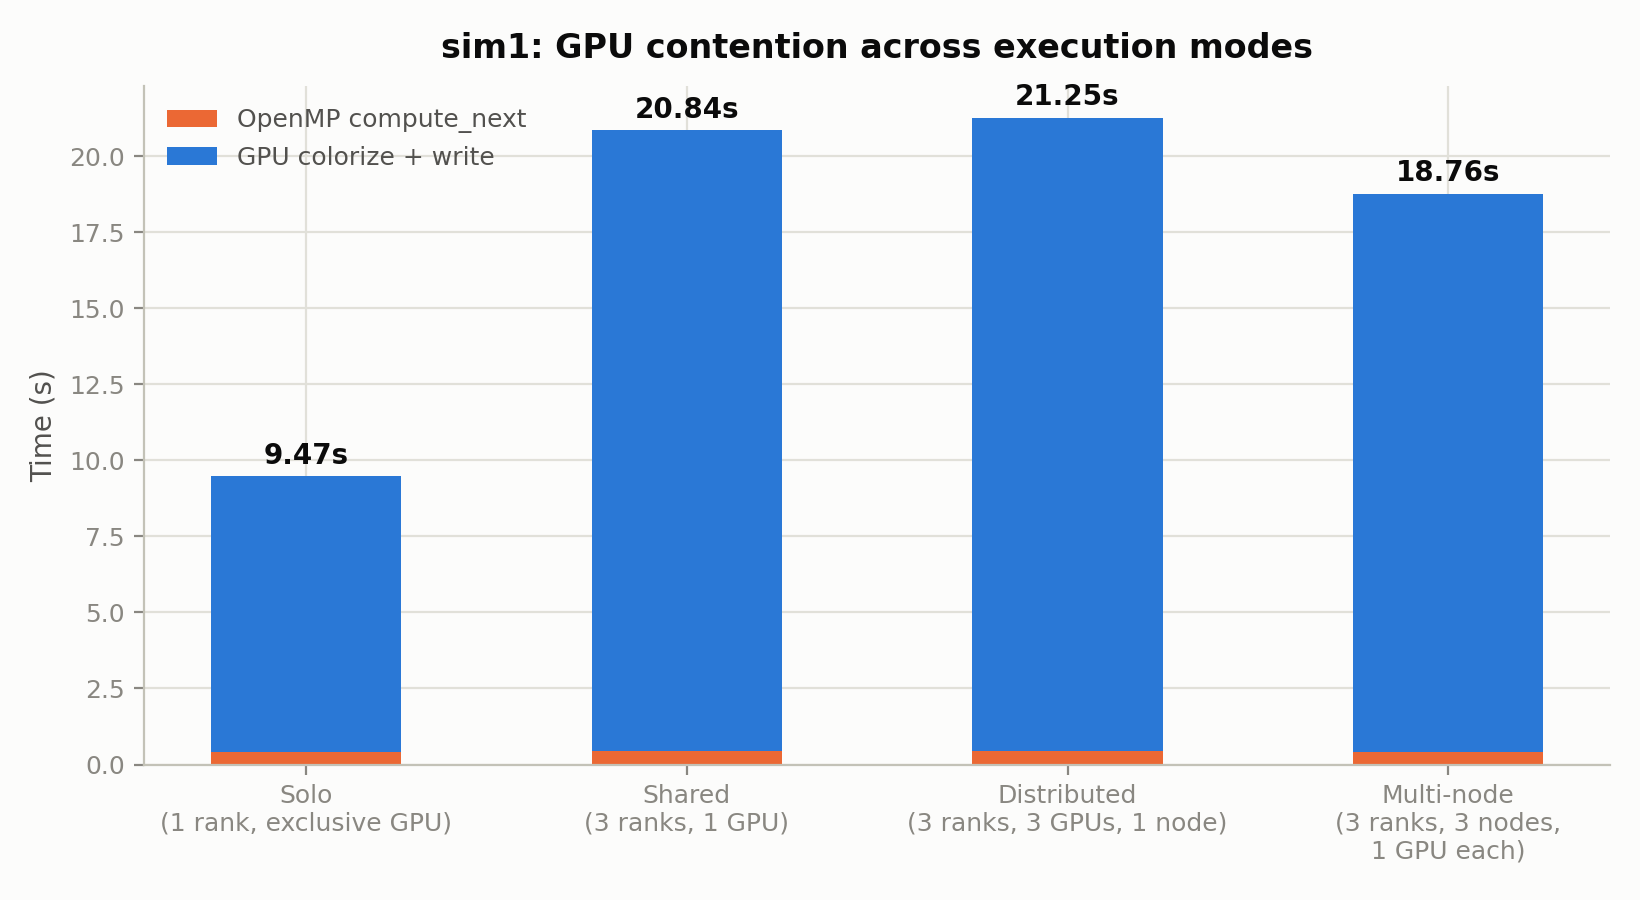
\includegraphics[width=0.6\textwidth]{../src/Davide/Final/Latex/figures/contention_sweep_solo_vs_shared.png}
    \caption{sim1's execution time across four GPU/node sharing configurations, identical workload.}
    \label{fig:contention}
\end{figure}

\subsection{Conclusions}
The dominant cost in this pipeline is not GPU compute (colorization
kernel: $\sim$1\% of frame time) nor CPU compute
(\texttt{compute\_next}: $\sim$2\%), but per-frame file I/O, specifically
whatever happens at \texttt{fclose} time rather than the write itself --
confirmed consistent across two GPU generations and reflected directly
in the GPU-sharing contention results: sharing the GPU across ranks
costs almost nothing, while sharing the filesystem costs a great deal.
This is the throughline of the whole investigation -- every optimization
decision was made only after measuring, not assumed from the physics
alone. Parallelizing the ASCII-formatting step was considered and
rejected once the phase breakdown showed it was $\sim$4\% of
\texttt{color\_time}, not worth the added complexity. Per-frame adaptive
color scaling was adopted only after raw pixel data confirmed a fixed
scale reads as pale almost immediately, since a 2D wave's peak amplitude
falls off geometrically with distance from the source on top of
$\gamma$-damping. And the GPU-sharing question itself was settled by
directly comparing four execution modes rather than assumed from GPU
specifications -- the result (I/O-bound, not compute-bound) held
consistently across every measurement in this report.

% -- report.tex already has graphicx/float in its preamble, and a shared
% report/b.bib for \cite{} (matching assignment_1's convention). All
% \includegraphics paths below are relative to report/, same as
% assignment_1/ass1.tex's own figures.

\section{Assignment 3}

\subsection{Introduction}
This assignment extends the damped wave simulator from parts 1--2 with
color. The physics, discretisation, and MPI/OpenMP structure are
unchanged: three MPI ranks each run one independent scenario (a single
impulse; two impulses starting together; two impulses with the second
delayed to $N/7$), each parallelised with OpenMP. What changes is the
output stage: each timestep's matrix is sent to the GPU, mapped to an RGB
triplet per pixel by a CUDA kernel, and saved as a P3 (ASCII) PPM frame
instead of a grayscale PGM. Bright, saturated colors mark the wave's
extrema, colors fade along the rising/falling fronts, and calm (near-zero)
regions are rendered white. 

%Student parameters (352165): $\gamma=0.067$,
%$c=0.59$, primary impulse at $(M/2,M/2)$ with amplitude 56; sim2's second
%wave at $(2M/3,M/4)$, amplitude $-35$, $t_{\mathrm{start}}=0$; sim3's second
%wave at $(M/3,M/3)$, amplitude 58, $t_{\mathrm{start}}=N/7$.
\subsection{Architecture}
The three MPI
ranks \cite{sanchezmpiintro} map naturally onto the three required
scenarios: each rank owns a complete, independent grid and runs one
scenario end to end, so the only collective call needed is a final
\texttt{MPI\_Allreduce} on success/failure. Within each rank, \texttt{compute\_next}
(the same 5-point Laplacian stencil as parts 1--2 -- each point's next
value is computed from itself and its 4 orthogonal neighbors via central
differences) is parallelised with OpenMP \cite{slidestatic}, using
\texttt{schedule(static)} for the same NUMA first-touch reason argued in
part 1: with a fixed thread-to-row mapping, the memory each thread first
writes (and therefore where the OS physically places it) matches the
memory that same thread repeatedly accesses on every subsequent call. After each timestep, the rank sends its
matrix to the GPU \cite{sanchezcuda}: a kernel normalizes each value
against the frame's own peak magnitude (found via a GPU-side reduction
\cite{sanchezgpuintro}), maps it to a color (white near zero, fading to
bright red/orange for positive values and blue for negative, saturating
at the wave's extrema), and the result is written to disk as an ASCII
PPM frame while the original scalar matrix continues to drive the
simulation.
Because the job requests a single GPU (\texttt{--gres=gpu:1}) for all
three ranks, the GPU is a shared resource -- a design point this report
returns to in Section~\ref{sec:contention}.

\subsection{Cluster hardware}
All experiments ran on Politecnico di Torino's HPC@PoliTO cluster
(Legion), specifically its EDU partitions -- reserved for coursework,
as opposed to the open-access or research-group-restricted partitions
also present on the cluster. Of the four EDU partitions, only two have
GPUs: \texttt{edu\_a40} and \texttt{edu\_v100}, confirmed live via
\texttt{sinfo -o "\%P \%D \%G"} (the other two, \texttt{edu\_skylake}
and \texttt{edu\_sapphire}, are CPU-only). \texttt{edu\_a40} nodes have 2 physical CPU sockets, 24 physical cores
per socket (48 physical cores/node), doubled to 96 logical cores/node by
SMT (2 hardware threads per core) -- confirmed via \texttt{sinfo}'s
socket/core/thread fields, since the cluster's own documentation lists
only the 48 physical cores -- and 4$\times$A40 GPUs;
\texttt{edu\_v100} nodes have 32 cores and 4$\times$V100 GPUs. Both are
used in this report: \texttt{edu\_a40} for all main results, and
\texttt{edu\_v100} as a cross-hardware check in Section~\ref{sec:nsys}.

\subsection{Metrics and the grid-size sweep}
\label{sec:metrics}
Beyond wall-clock time, the program times two phases directly:
\texttt{color\_time} (GPU colorization + PPM write, per frame) and
\texttt{compute\_time} (the OpenMP stencil update). \texttt{color\_time}
is further split into five sub-phases -- H2D copy, kernel, D2H copy,
ASCII formatting, and disk write -- introduced in
Section~\ref{sec:phase}. Figure~\ref{fig:size} sweeps grid size $M$ from
128 to 4096 (\texttt{edu\_a40}, 4 threads, 50 steps). Execution time
approaches ideal $O(M^2)$ scaling as $M$ grows: $128\to256$ costs only
$2.1\times$ (fixed per-run overhead still dominant at small $M$), while
$2048\to4096$ costs $4.1\times$ -- essentially the ideal quadratic ratio.
The right panel shows GPU colorize+write dominating total time
throughout: at $M=4096$ it is $\sim$97.6\% of total time, versus
\texttt{compute\_next} at $\sim$2.4\%. Both phases are $O(M^2)$, so this
ratio stays roughly constant across the whole sweep ($\sim$97.6--97.7\%
from $M=256$ upward; only the smallest grid, $M=128$, deviates, where
fixed per-run overhead is large enough to matter).

We capped the sweep at $M=4096$ rather than matching part 1's $M=15000$:
at $M=4096$ an ASCII PPM frame is already $\sim$100--130MB, so scaling to
$M=15000$ -- $(15000/4096)^2\approx13\times$ the pixels -- would push
single frames into the multi-gigabyte range across 50 steps and 3 ranks,
for a sweep whose purpose (showing execution time approach ideal
$O(M^2)$ scaling and locating the point where GPU colorize+write comes
to dominate) was already unambiguous well before $M=4096$.

\begin{figure}[h]
    \centering
    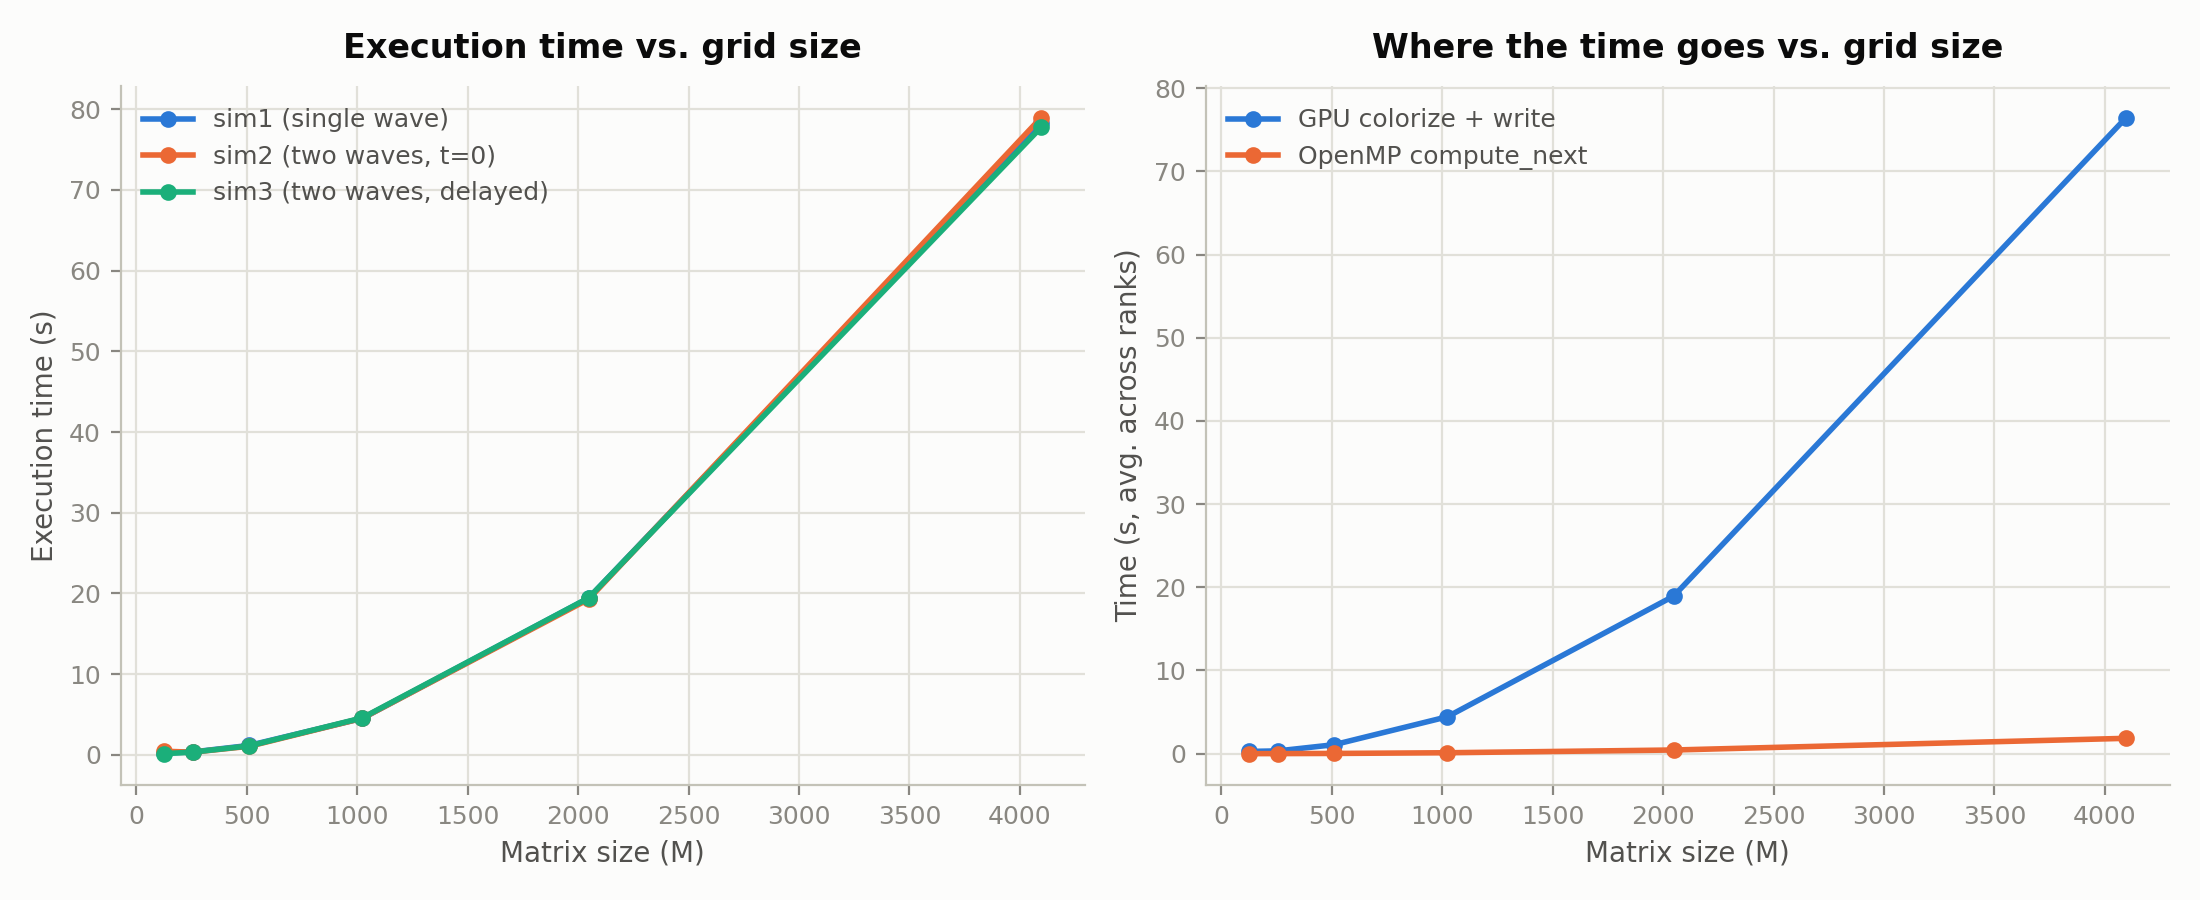
\includegraphics[width=0.68\textwidth]{../src/Davide/Final/Latex/figures/size_sweep_execution_time.png}
    \caption{Execution time and its GPU/OpenMP split, varying grid size $M$ (4 threads, 3 ranks sharing 1 GPU).}
    \label{fig:size}
\end{figure}

\subsection{Phase breakdown: is the ASCII formatting worth parallelizing?}
\label{sec:phase}
Figure~\ref{fig:phase} breaks \texttt{color\_time} into its five
sub-phases. At $M=4096$ (averaged over 3 ranks): \texttt{write} (the
\texttt{fwrite} call) is $\sim$94.6\% of \texttt{color\_time},
\texttt{format} (the ASCII byte-to-digit conversion) is $\sim$4.3\%, and
H2D copy + kernel + D2H copy combined are $\sim$1\%. The same lopsided
pattern holds at every grid size swept, not only at $M=4096$.

This directly answers a question we considered early on: is it worth
parallelizing the ASCII-formatting step with OpenMP? It is not --
formatting is only $\sim$4\% of \texttt{color\_time}, so even a
theoretical zero-overhead parallelization would save a few percent of
total time at best, not worth the added complexity (the output is
variable-width per pixel, so parallel writers would need either a
prefix-sum pass to compute offsets first, or a switch to fixed-width
padding). We measured before optimizing, and the measurement said no.

\begin{figure}[h]
    \centering
    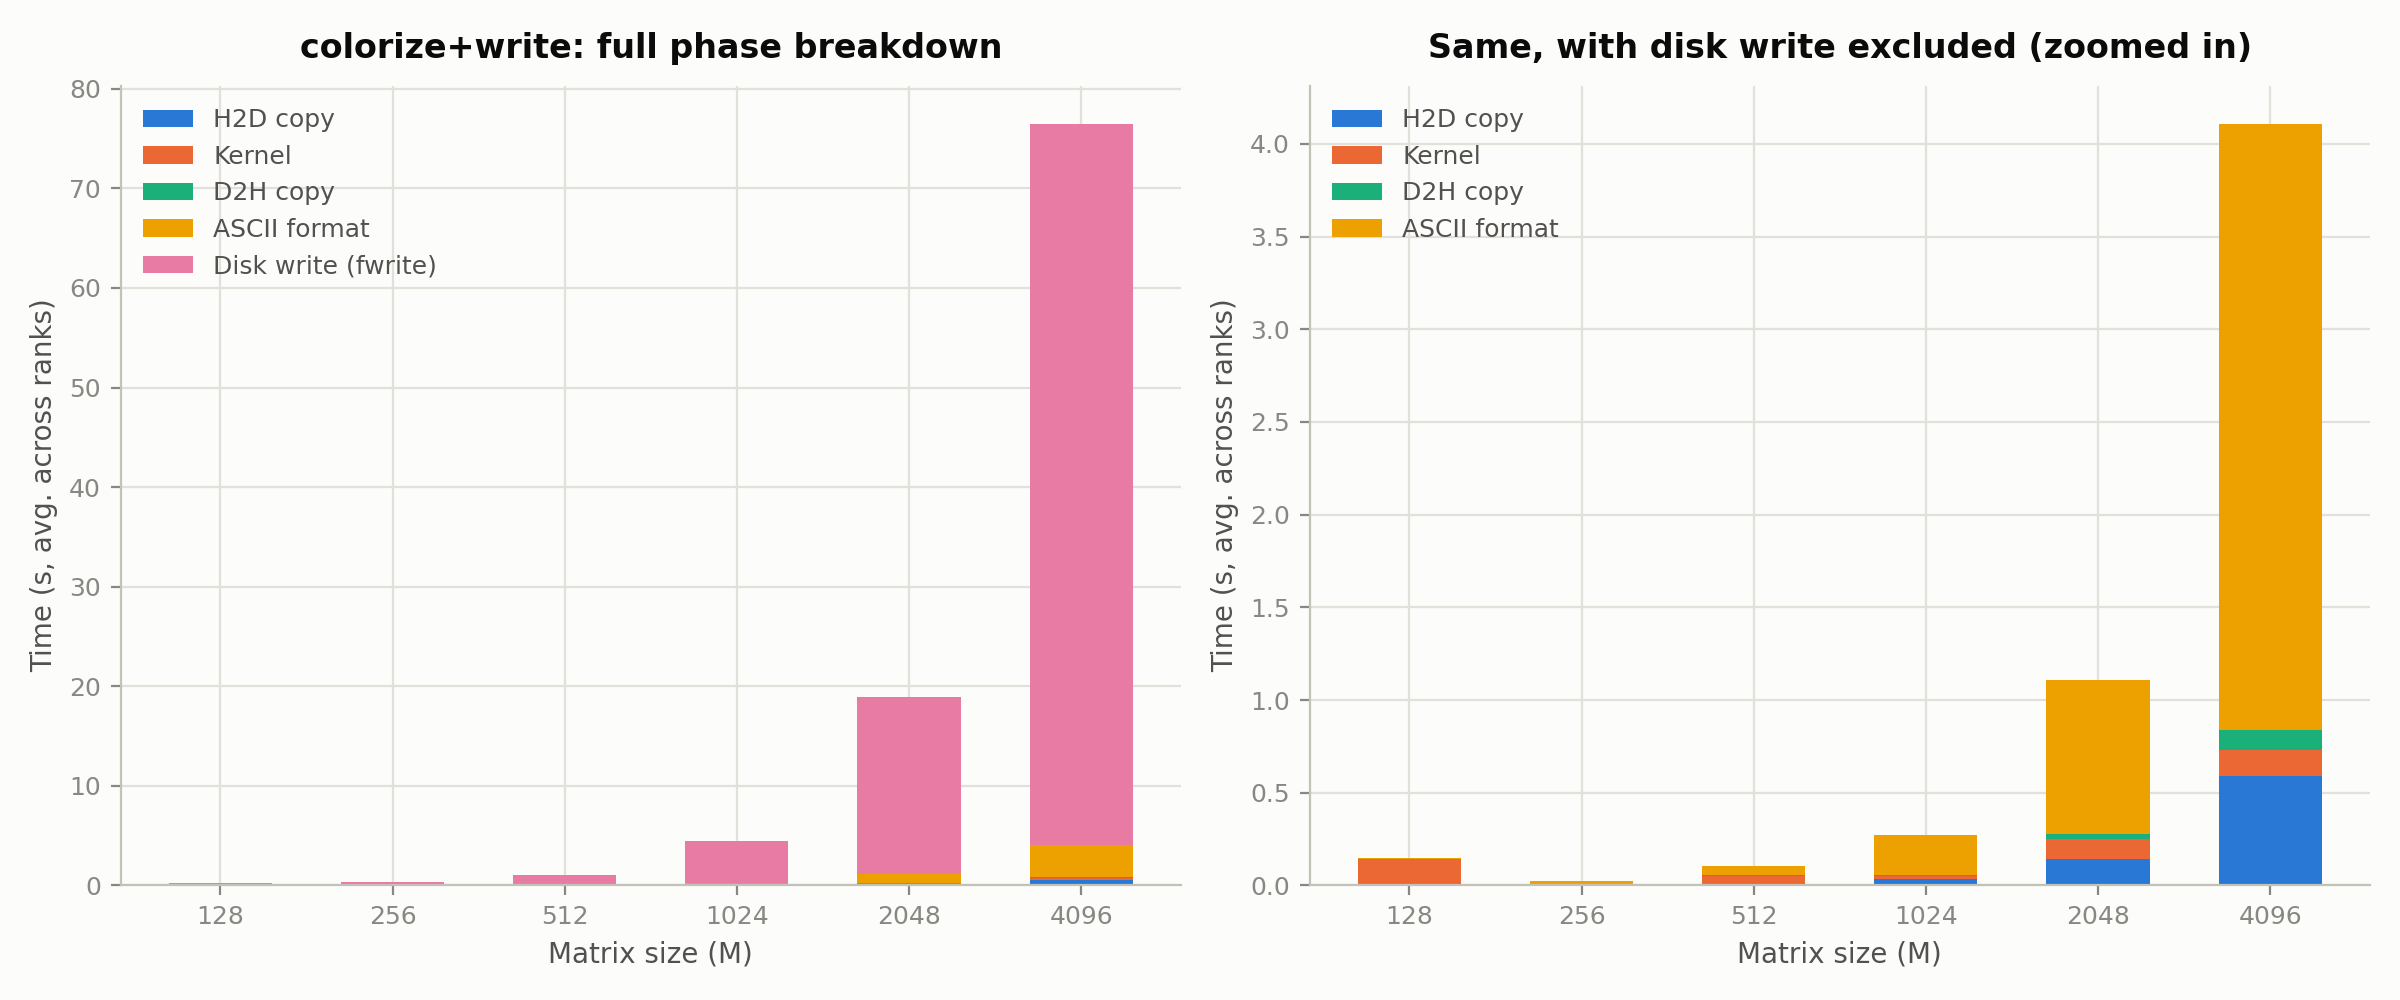
\includegraphics[width=0.68\textwidth]{../src/Davide/Final/Latex/figures/size_sweep_phase_breakdown.png}
    \caption{colorize+write split into its 5 phases vs.\ grid size. Left: full stack (write's dominance is the point, not log-scaled). Right: same data with write excluded, zoomed in.}
    \label{fig:phase}
\end{figure}

\subsection{Where does the write time actually go? Nsight Systems, cross-checked on two GPUs}
\label{sec:nsys}
Nsight Compute (kernel-level occupancy/throughput metrics) was
attempted but is unavailable on this cluster: it returns
\texttt{ERR\_NVGPUCTRPERM} -- GPU performance-counter access is
admin-only, a driver-level restriction no user-side flag can work
around. Nsight Systems was used instead, and it revealed something our
own coarse \texttt{write\_s} timer could not: that timer wraps
\texttt{fopen}+\texttt{fwrite}+\texttt{fclose} as one block, and Nsight
Systems' OS Runtime Summary lets us split it apart. On \texttt{edu\_a40}:
\texttt{fwrite} itself is cheap ($\sim$0.6\% of total OS-runtime time),
while \texttt{fclose} is $\sim$18.3\% -- roughly 30$\times$ more
expensive than the write call it follows. The two largest categories by
far, \texttt{epoll\_wait} ($\sim$52\%) and \texttt{poll} ($\sim$25\%), we
initially guessed reflected ranks idling on MPI's progress engine. A
follow-up run with MPI event tracing enabled rules that out directly:
summed across \texttt{MPI\_Init}, \texttt{MPI\_Finalize}, and the one
real collective (\texttt{MPI\_Allreduce}), application-level MPI time is
$\sim$0.56s per rank -- under 2\% of the combined
\texttt{epoll\_wait}+\texttt{poll} time ($\sim$28.4s). \texttt{MPI\_Allreduce}
itself is 13.7ms. The better-supported explanation, from a companion
VTune Threading run on the same job: its top wait objects include
InfiniBand verbs streams (\texttt{/dev/infiniband/uverbs0}), suggesting
OpenMPI's UCX transport stack is initialized and idly polling in the
background for the whole process lifetime regardless of how little it is
actually used -- not the application's own collective calls, but the
runtime's transport layer underneath them. We report this as the
better-supported hypothesis, not a fully isolated cause. To check whether the OS-runtime pattern itself is an artifact of
one specific GPU, we repeated the identical run on \texttt{edu\_v100} --
an older GPU generation with a slower host interconnect (the whole
production run was $\sim$3$\times$ slower end-to-end on V100, consistent
with H2D transfer time alone rising from $\sim$52\% to $\sim$67\% of GPU
time). Despite the large hardware difference, the OS-runtime split is
nearly identical (Figure~\ref{fig:nsys}): \texttt{fclose} $\sim$17.9\%,
\texttt{fwrite} $\sim$0.4\%, \texttt{epoll\_wait}+\texttt{poll}
$\sim$76\% combined on both. This is good evidence the bottleneck is
I/O/synchronization behavior, not GPU-specific.

\begin{figure}[h]
    \centering
    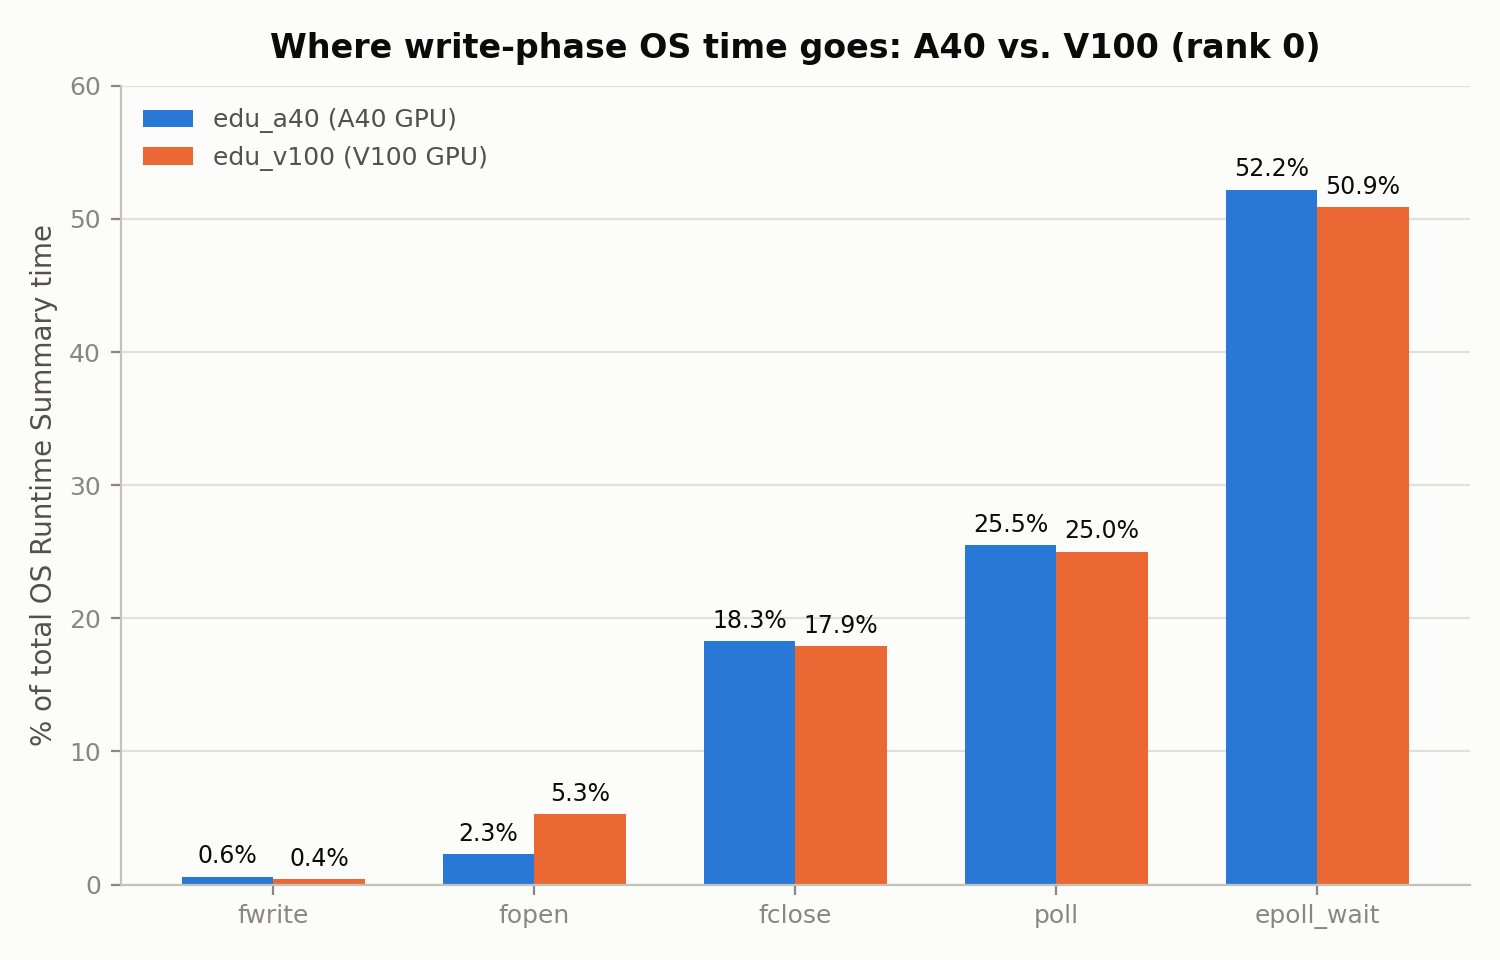
\includegraphics[width=0.6\textwidth]{../src/Davide/Final/Latex/figures/nsys_os_runtime_breakdown.png}
    \caption{OS Runtime Summary breakdown (rank 0), \texttt{edu\_a40} vs.\ \texttt{edu\_v100} -- nearly identical despite very different GPU hardware.}
    \label{fig:nsys}
\end{figure}

\subsection{OpenMP thread scaling and CUDA block size}
Figure~\ref{fig:thread} sweeps OpenMP thread count 1--32 at $M=4096$ (the
full logical-core range of one \texttt{edu\_a40} rank, $96/3$). Both the
full-pipeline and \texttt{compute\_next}-only curves are essentially
flat, never exceeding $\sim$1.2$\times$ speedup, with compute-only
plateauing by 2 threads and staying flat through 32. This is consistent
with the 5-point stencil being memory-bandwidth-bound rather than
compute-bound (4 loads, 1 store, few FLOPs per point) -- a small number
of threads already saturates available memory bandwidth. We also
considered an alternative explanation -- that \texttt{compute\_next}
forking a fresh OpenMP thread team on every one of 300 calls/rank could
plateau this curve through fork/join overhead alone, independent of
memory bandwidth -- and ruled it out with VTune Hotspots at $M=4096$:
\texttt{gomp\_team\_barrier\_wait\_end} does not appear among the top
hotspots at either 4 or 32 threads (unlike part 1's profile, where it was
79.4\% of CPU time), and \texttt{compute\_next}'s own CPU time is flat
across that range (3.43s at 4 threads vs.\ 3.21s at 32) rather than
growing with team size. This contrasts
with part 1's own OpenMP results, which showed real scaling at large
thread counts, mainly because part 1 tested $M$ up to 15000 -- large
enough for the stencil's absolute cost to be interesting on its own,
with no competing GPU-bound stage.

\begin{figure}[h]
    \centering
    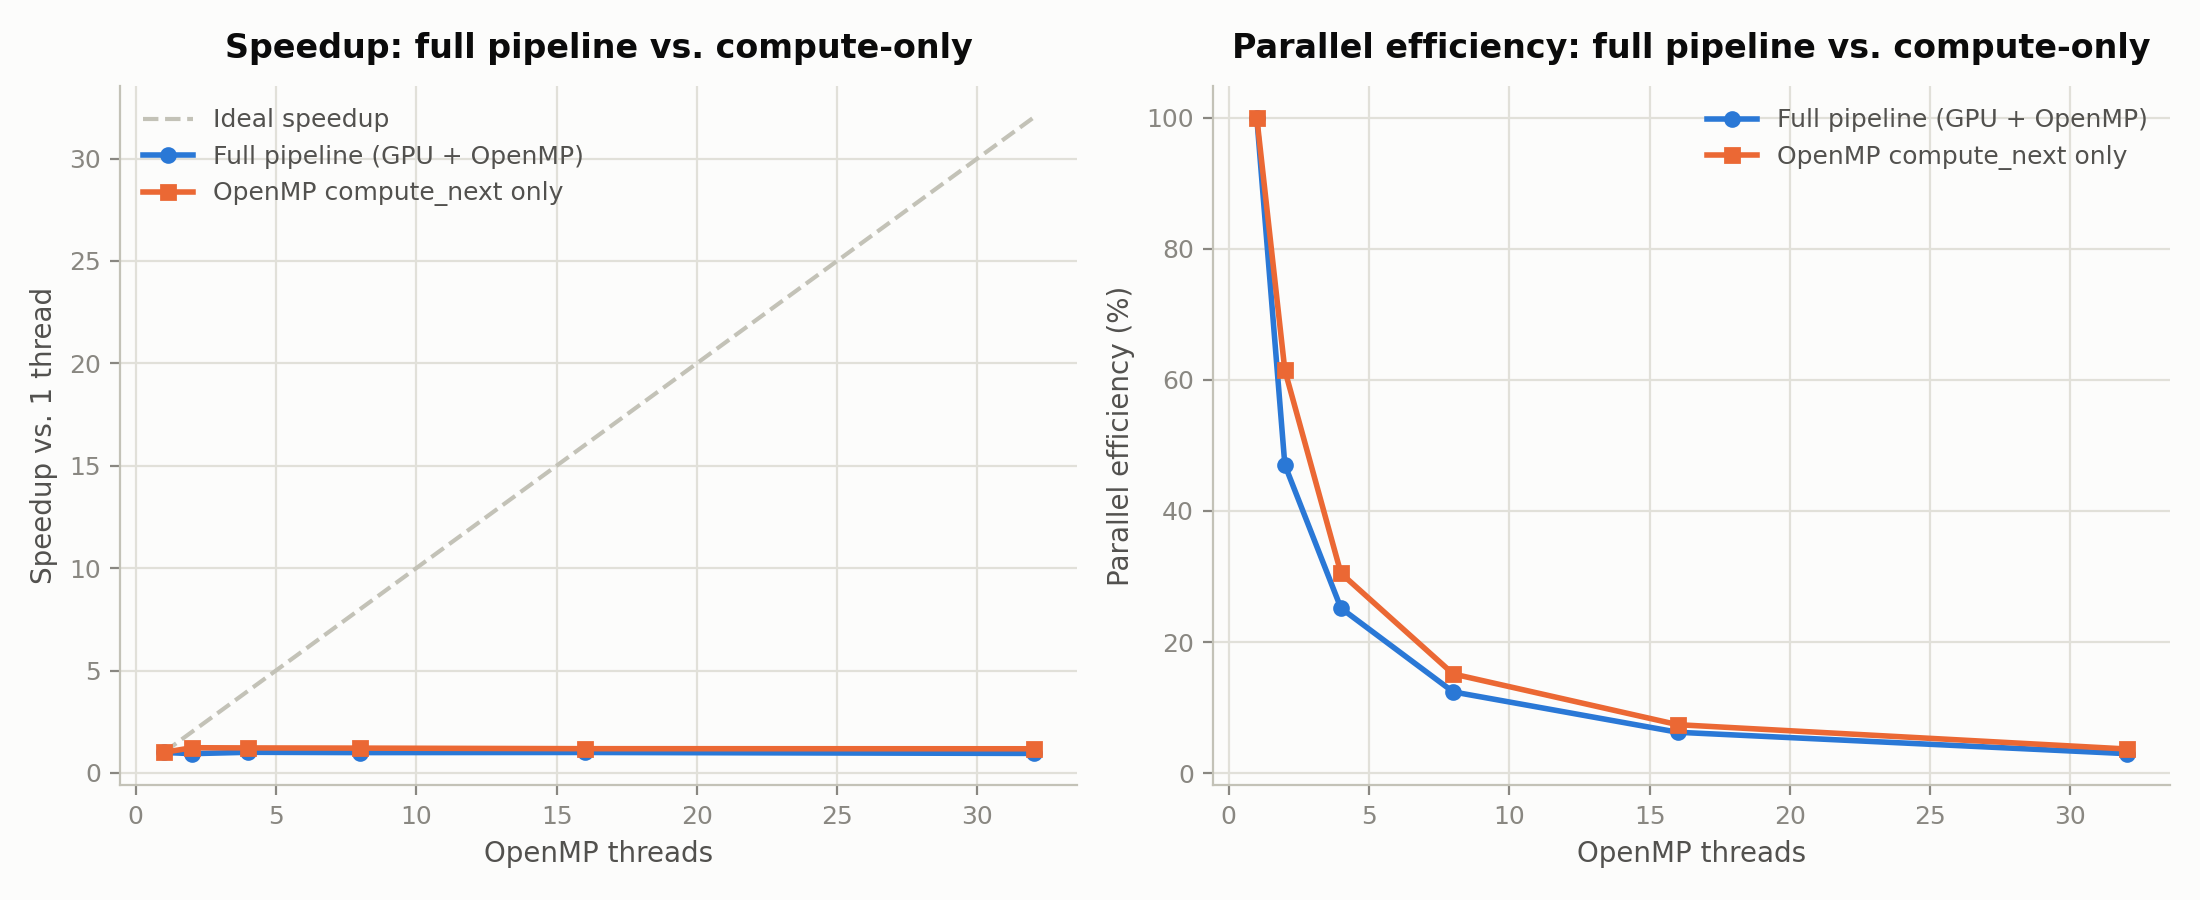
\includegraphics[width=0.68\textwidth]{../src/Davide/Final/Latex/figures/thread_sweep_speedup_efficiency.png}
    \caption{Speedup and efficiency vs.\ OpenMP thread count at $M=4096$, full pipeline vs.\ compute-only.}
    \label{fig:thread}
\end{figure}

Figure~\ref{fig:block} sweeps the CUDA kernel's threads-per-block at
$M=4096$: time decreases roughly monotonically as block size grows,
worst at 32 threads/block ($\sim$83s average) and best at 1024
($\sim$73s, $\sim$12\% faster), with only a minor plateau between 128
and 512. Since Nsight Compute (the tool that would report actual
occupancy) is unavailable on this cluster, we do not have a
profiler-level explanation for this trend, only the timing result
itself -- the most we can say is that fewer, larger blocks amortize
per-block launch and scheduling overhead across more threads. A smaller,
noisier earlier sweep at $M=1024$ (not shown) trended the opposite way
at the high end, so we do not treat this shape as independently
confirmed and report only the $M=4096$ result.

\begin{figure}[h]
    \centering
    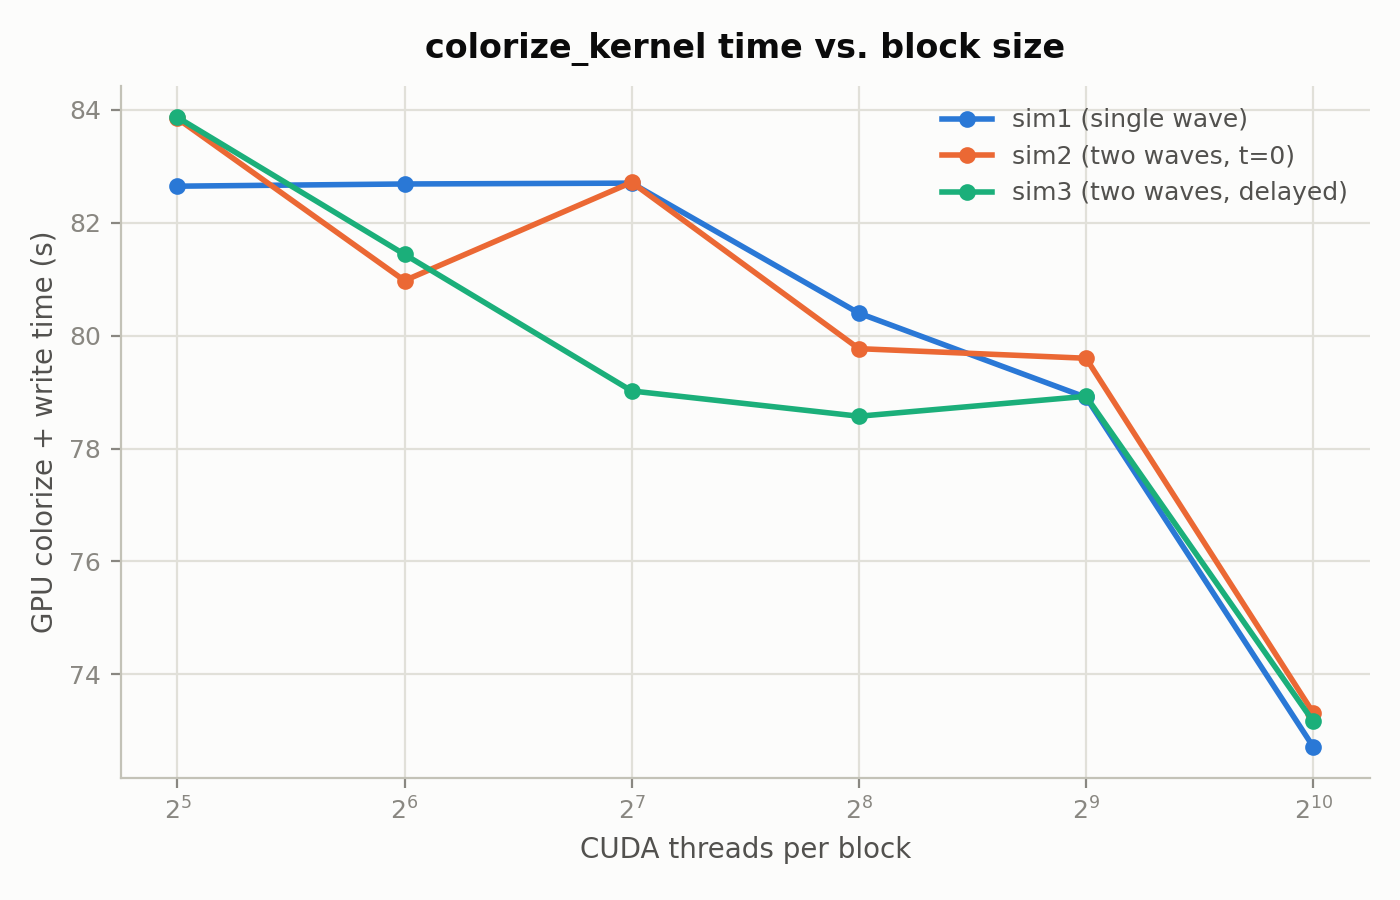
\includegraphics[width=0.52\textwidth]{../src/Davide/Final/Latex/figures/blocksize_sweep_kernel_time.png}
    \caption{GPU colorize+write time vs.\ CUDA threads-per-block, $M=4096$.}
    \label{fig:block}
\end{figure}

\subsection{GPU contention across execution modes}
\label{sec:contention}
Section~\ref{sec:phase} showed disk writes dominate; this raises the
question of how much the design choice of sharing one GPU across 3
ranks actually costs. We compared four execution modes at identical
parameters ($M=2048$, 50 steps, 4 threads), isolating sim1's workload
in each: \texttt{solo} (1 rank, exclusive GPU), \texttt{shared} (the
normal 3-rank/1-GPU run), \texttt{distributed} (3 ranks, 3 dedicated
GPUs on one node, \texttt{--gres=gpu:3}), and \texttt{multinode} (3
ranks on 3 separate nodes, one dedicated GPU each, communicating over
the cluster's Infiniband fabric \cite{sanchezmpitopo}). Results
(Figure~\ref{fig:contention}): \texttt{solo} 9.47s, \texttt{shared}
20.84s, \texttt{distributed} 21.25s, \texttt{multinode} 18.76s.

Two findings. First, dedicating a GPU per rank alone
(\texttt{distributed} vs.\ \texttt{shared}) makes no reliable difference
at all -- \texttt{distributed} is actually $\sim$2\% \emph{slower} here,
well within run-to-run noise rather than a real effect either way --
GPU compute-engine time-slicing is not the bottleneck. Second,
\texttt{solo} is dramatically faster than every multi-rank mode (roughly
half the time, $\sim$50--55\% less depending on which mode it's compared
against), which Section~\ref{sec:phase}'s finding
explains directly: \texttt{shared} and \texttt{distributed} both have 3
ranks writing frames \emph{concurrently} to the same node; \texttt{solo}
is the only mode with exactly one writer at a time, anywhere.
\texttt{multinode} sits in between ($\sim$10\% faster than
\texttt{distributed}) by removing host-local contention (memory bus,
PCIe root complex) but not, most plausibly, a deeper one: all three
nodes most likely still write to the same shared, network-attached
storage behind every node's home directory (per the cluster's own
documentation, though not measured directly here) -- the best available
explanation for why multinode sits closer to \texttt{shared} than to
\texttt{solo}. The dominant contention in this workload is concurrent
I/O, not GPU compute-engine sharing -- consistent with
Section~\ref{sec:nsys}'s \texttt{fclose}-dominated OS Runtime profile.

\begin{figure}[h]
    \centering
    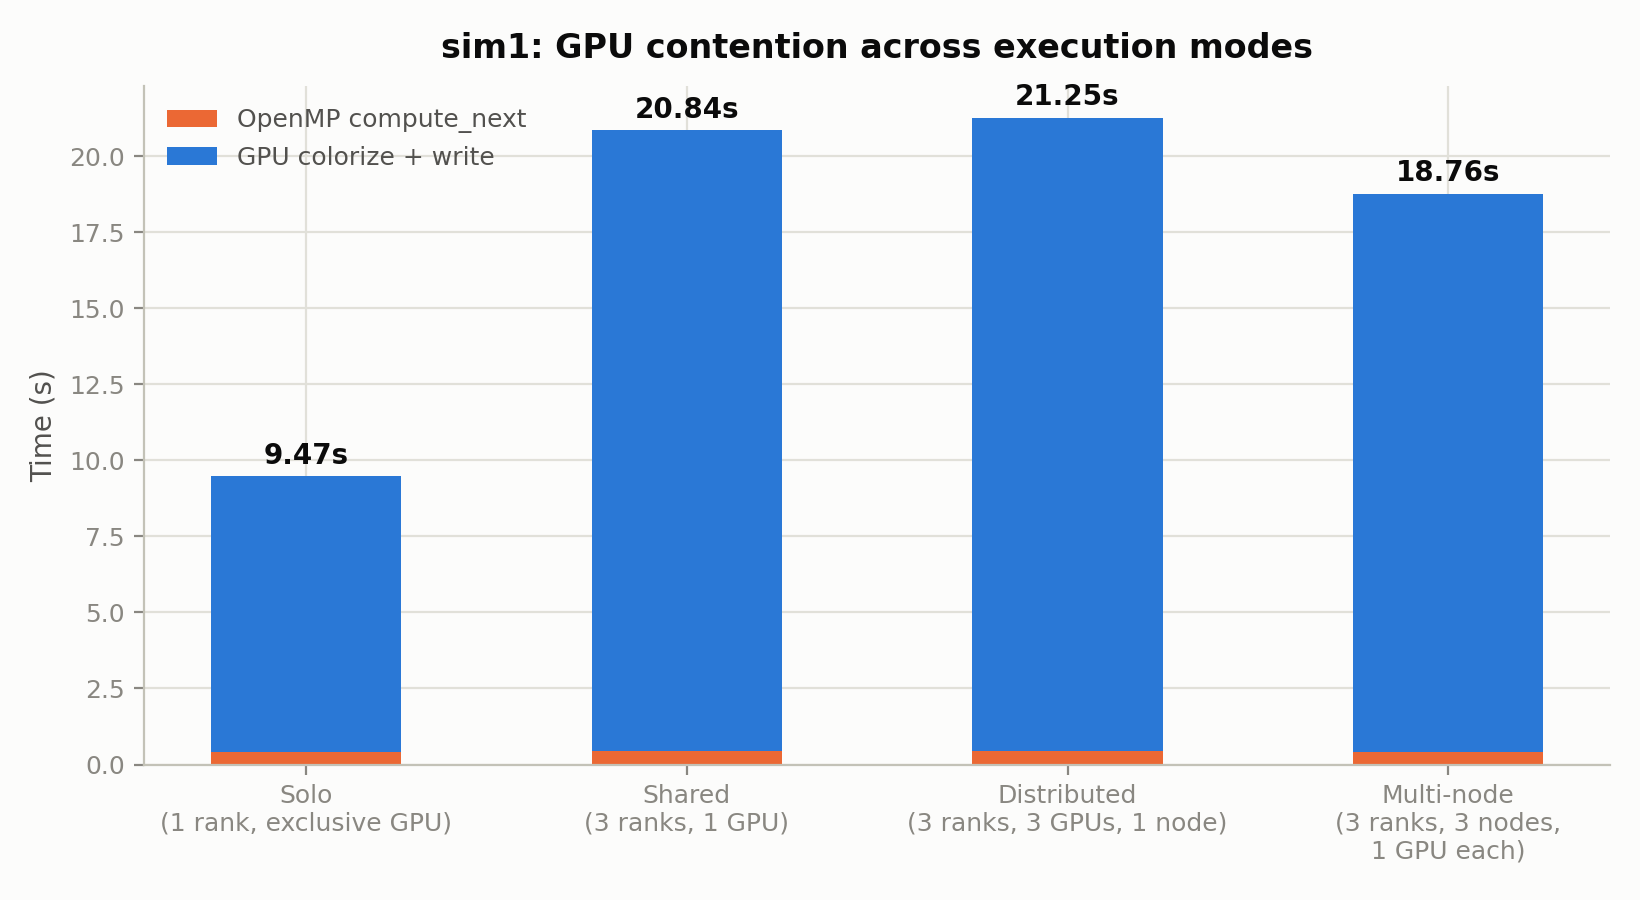
\includegraphics[width=0.6\textwidth]{../src/Davide/Final/Latex/figures/contention_sweep_solo_vs_shared.png}
    \caption{sim1's execution time across four GPU/node sharing configurations, identical workload.}
    \label{fig:contention}
\end{figure}

\subsection{Conclusions}
The dominant cost in this pipeline is not GPU compute (colorization
kernel: $\sim$1\% of frame time) nor CPU compute
(\texttt{compute\_next}: $\sim$2\%), but per-frame file I/O, specifically
whatever happens at \texttt{fclose} time rather than the write itself --
confirmed consistent across two GPU generations and reflected directly
in the GPU-sharing contention results: sharing the GPU across ranks
costs almost nothing, while sharing the filesystem costs a great deal.
This is the throughline of the whole investigation -- every optimization
decision was made only after measuring, not assumed from the physics
alone. Parallelizing the ASCII-formatting step was considered and
rejected once the phase breakdown showed it was $\sim$4\% of
\texttt{color\_time}, not worth the added complexity. Per-frame adaptive
color scaling was adopted only after raw pixel data confirmed a fixed
scale reads as pale almost immediately, since a 2D wave's peak amplitude
falls off geometrically with distance from the source on top of
$\gamma$-damping. And the GPU-sharing question itself was settled by
directly comparing four execution modes rather than assumed from GPU
specifications -- the result (I/O-bound, not compute-bound) held
consistently across every measurement in this report.

% -- report.tex already has graphicx/float in its preamble, and a shared
% report/b.bib for \cite{} (matching assignment_1's convention). All
% \includegraphics paths below are relative to report/, same as
% assignment_1/ass1.tex's own figures.

\section{Assignment 3}

\subsection{Introduction}
This assignment extends the damped wave simulator from parts 1--2 with
color. The physics, discretisation, and MPI/OpenMP structure are
unchanged: three MPI ranks each run one independent scenario (a single
impulse; two impulses starting together; two impulses with the second
delayed to $N/7$), each parallelised with OpenMP. What changes is the
output stage: each timestep's matrix is sent to the GPU, mapped to an RGB
triplet per pixel by a CUDA kernel, and saved as a P3 (ASCII) PPM frame
instead of a grayscale PGM. Bright, saturated colors mark the wave's
extrema, colors fade along the rising/falling fronts, and calm (near-zero)
regions are rendered white. 

%Student parameters (352165): $\gamma=0.067$,
%$c=0.59$, primary impulse at $(M/2,M/2)$ with amplitude 56; sim2's second
%wave at $(2M/3,M/4)$, amplitude $-35$, $t_{\mathrm{start}}=0$; sim3's second
%wave at $(M/3,M/3)$, amplitude 58, $t_{\mathrm{start}}=N/7$.
\subsection{Architecture}
The three MPI
ranks \cite{sanchezmpiintro} map naturally onto the three required
scenarios: each rank owns a complete, independent grid and runs one
scenario end to end, so the only collective call needed is a final
\texttt{MPI\_Allreduce} on success/failure. Within each rank, \texttt{compute\_next}
(the same 5-point Laplacian stencil as parts 1--2 -- each point's next
value is computed from itself and its 4 orthogonal neighbors via central
differences) is parallelised with OpenMP \cite{slidestatic}, using
\texttt{schedule(static)} for the same NUMA first-touch reason argued in
part 1: with a fixed thread-to-row mapping, the memory each thread first
writes (and therefore where the OS physically places it) matches the
memory that same thread repeatedly accesses on every subsequent call. After each timestep, the rank sends its
matrix to the GPU \cite{sanchezcuda}: a kernel normalizes each value
against the frame's own peak magnitude (found via a GPU-side reduction
\cite{sanchezgpuintro}), maps it to a color (white near zero, fading to
bright red/orange for positive values and blue for negative, saturating
at the wave's extrema), and the result is written to disk as an ASCII
PPM frame while the original scalar matrix continues to drive the
simulation.
Because the job requests a single GPU (\texttt{--gres=gpu:1}) for all
three ranks, the GPU is a shared resource -- a design point this report
returns to in Section~\ref{sec:contention}.

\subsection{Cluster hardware}
All experiments ran on Politecnico di Torino's HPC@PoliTO cluster
(Legion), specifically its EDU partitions -- reserved for coursework,
as opposed to the open-access or research-group-restricted partitions
also present on the cluster. Of the four EDU partitions, only two have
GPUs: \texttt{edu\_a40} and \texttt{edu\_v100}, confirmed live via
\texttt{sinfo -o "\%P \%D \%G"} (the other two, \texttt{edu\_skylake}
and \texttt{edu\_sapphire}, are CPU-only). \texttt{edu\_a40} nodes have 2 physical CPU sockets, 24 physical cores
per socket (48 physical cores/node), doubled to 96 logical cores/node by
SMT (2 hardware threads per core) -- confirmed via \texttt{sinfo}'s
socket/core/thread fields, since the cluster's own documentation lists
only the 48 physical cores -- and 4$\times$A40 GPUs;
\texttt{edu\_v100} nodes have 32 cores and 4$\times$V100 GPUs. Both are
used in this report: \texttt{edu\_a40} for all main results, and
\texttt{edu\_v100} as a cross-hardware check in Section~\ref{sec:nsys}.

\subsection{Metrics and the grid-size sweep}
\label{sec:metrics}
Beyond wall-clock time, the program times two phases directly:
\texttt{color\_time} (GPU colorization + PPM write, per frame) and
\texttt{compute\_time} (the OpenMP stencil update). \texttt{color\_time}
is further split into five sub-phases -- H2D copy, kernel, D2H copy,
ASCII formatting, and disk write -- introduced in
Section~\ref{sec:phase}. Figure~\ref{fig:size} sweeps grid size $M$ from
128 to 4096 (\texttt{edu\_a40}, 4 threads, 50 steps). Execution time
approaches ideal $O(M^2)$ scaling as $M$ grows: $128\to256$ costs only
$2.1\times$ (fixed per-run overhead still dominant at small $M$), while
$2048\to4096$ costs $4.1\times$ -- essentially the ideal quadratic ratio.
The right panel shows GPU colorize+write dominating total time
throughout: at $M=4096$ it is $\sim$97.6\% of total time, versus
\texttt{compute\_next} at $\sim$2.4\%. Both phases are $O(M^2)$, so this
ratio stays roughly constant across the whole sweep ($\sim$97.6--97.7\%
from $M=256$ upward; only the smallest grid, $M=128$, deviates, where
fixed per-run overhead is large enough to matter).

We capped the sweep at $M=4096$ rather than matching part 1's $M=15000$:
at $M=4096$ an ASCII PPM frame is already $\sim$100--130MB, so scaling to
$M=15000$ -- $(15000/4096)^2\approx13\times$ the pixels -- would push
single frames into the multi-gigabyte range across 50 steps and 3 ranks,
for a sweep whose purpose (showing execution time approach ideal
$O(M^2)$ scaling and locating the point where GPU colorize+write comes
to dominate) was already unambiguous well before $M=4096$.

\begin{figure}[h]
    \centering
    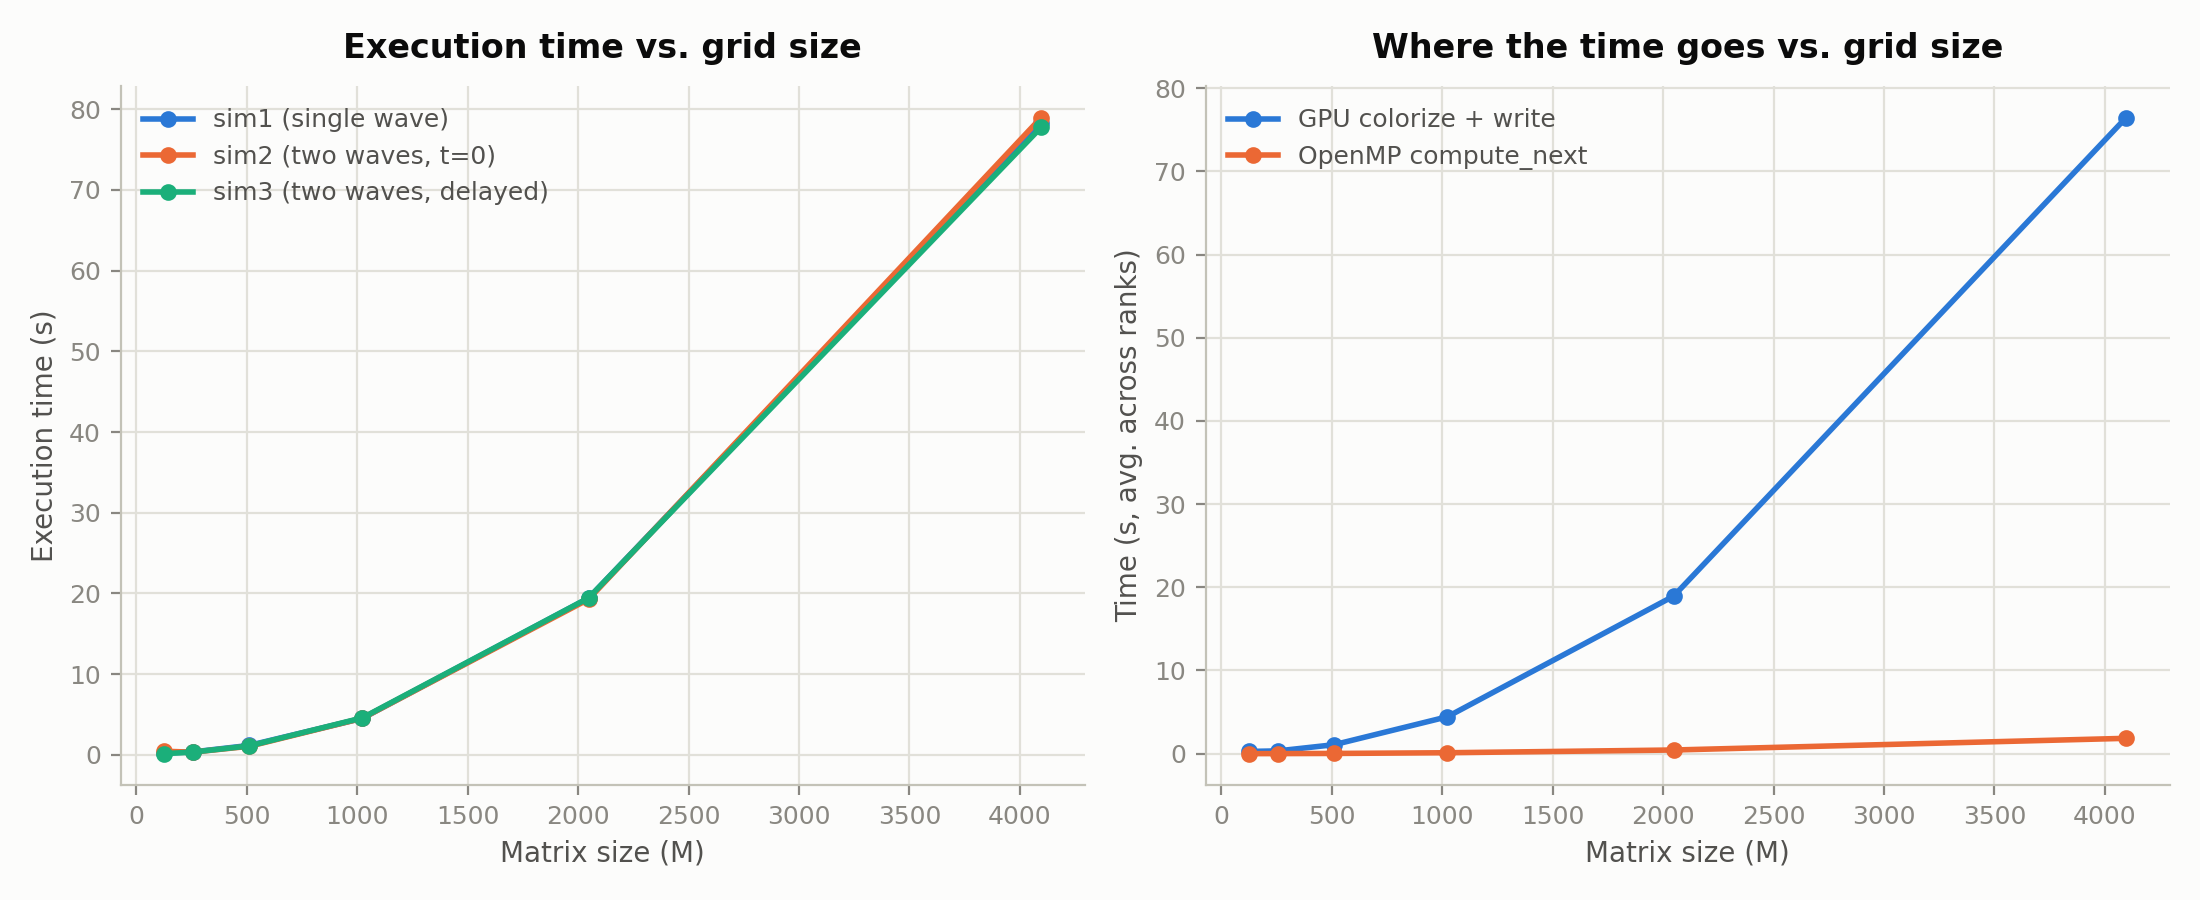
\includegraphics[width=0.68\textwidth]{../src/Davide/Final/Latex/figures/size_sweep_execution_time.png}
    \caption{Execution time and its GPU/OpenMP split, varying grid size $M$ (4 threads, 3 ranks sharing 1 GPU).}
    \label{fig:size}
\end{figure}

\subsection{Phase breakdown: is the ASCII formatting worth parallelizing?}
\label{sec:phase}
Figure~\ref{fig:phase} breaks \texttt{color\_time} into its five
sub-phases. At $M=4096$ (averaged over 3 ranks): \texttt{write} (the
\texttt{fwrite} call) is $\sim$94.6\% of \texttt{color\_time},
\texttt{format} (the ASCII byte-to-digit conversion) is $\sim$4.3\%, and
H2D copy + kernel + D2H copy combined are $\sim$1\%. The same lopsided
pattern holds at every grid size swept, not only at $M=4096$.

This directly answers a question we considered early on: is it worth
parallelizing the ASCII-formatting step with OpenMP? It is not --
formatting is only $\sim$4\% of \texttt{color\_time}, so even a
theoretical zero-overhead parallelization would save a few percent of
total time at best, not worth the added complexity (the output is
variable-width per pixel, so parallel writers would need either a
prefix-sum pass to compute offsets first, or a switch to fixed-width
padding). We measured before optimizing, and the measurement said no.

\begin{figure}[h]
    \centering
    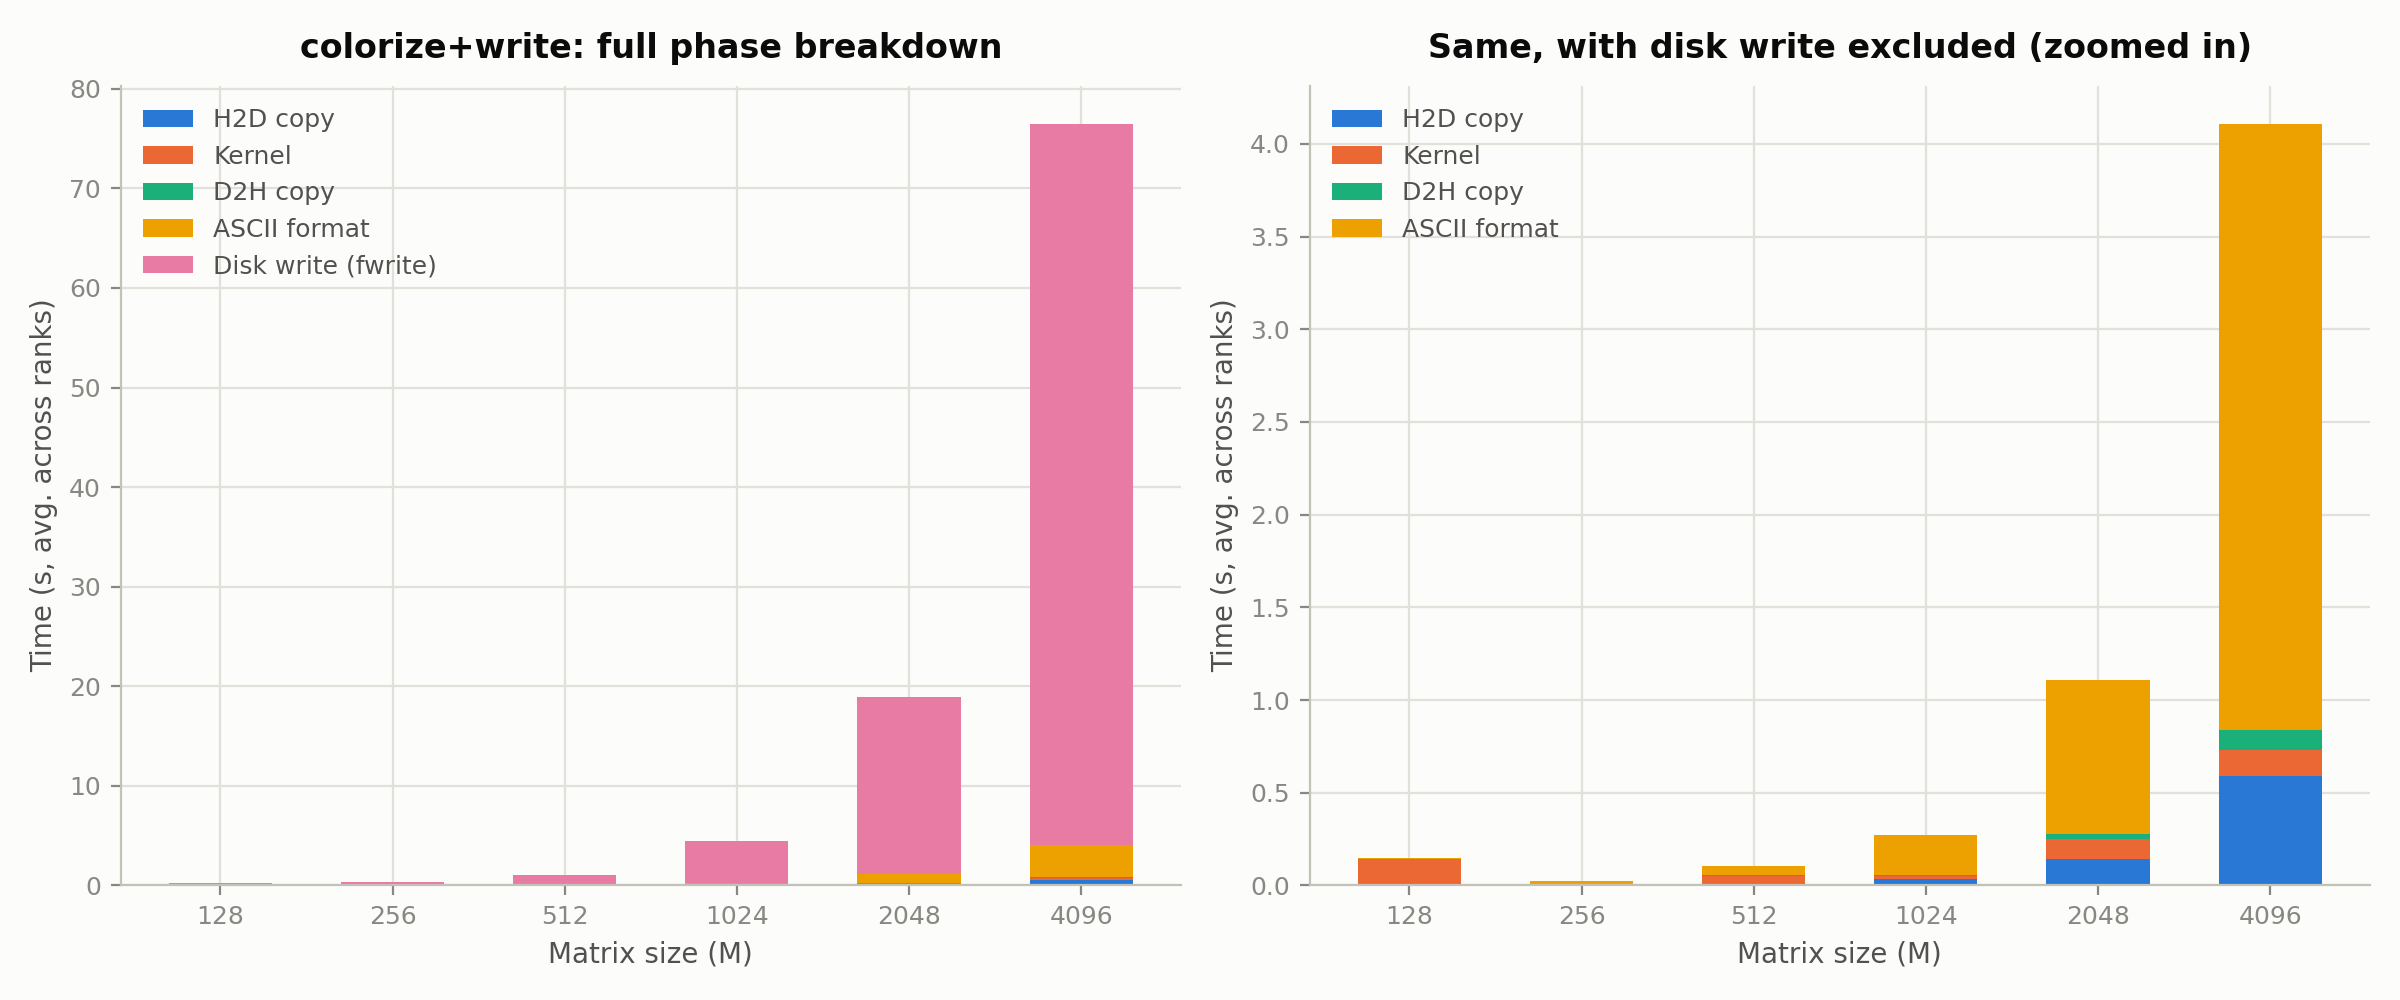
\includegraphics[width=0.68\textwidth]{../src/Davide/Final/Latex/figures/size_sweep_phase_breakdown.png}
    \caption{colorize+write split into its 5 phases vs.\ grid size. Left: full stack (write's dominance is the point, not log-scaled). Right: same data with write excluded, zoomed in.}
    \label{fig:phase}
\end{figure}

\subsection{Where does the write time actually go? Nsight Systems, cross-checked on two GPUs}
\label{sec:nsys}
Nsight Compute (kernel-level occupancy/throughput metrics) was
attempted but is unavailable on this cluster: it returns
\texttt{ERR\_NVGPUCTRPERM} -- GPU performance-counter access is
admin-only, a driver-level restriction no user-side flag can work
around. Nsight Systems was used instead, and it revealed something our
own coarse \texttt{write\_s} timer could not: that timer wraps
\texttt{fopen}+\texttt{fwrite}+\texttt{fclose} as one block, and Nsight
Systems' OS Runtime Summary lets us split it apart. On \texttt{edu\_a40}:
\texttt{fwrite} itself is cheap ($\sim$0.6\% of total OS-runtime time),
while \texttt{fclose} is $\sim$18.3\% -- roughly 30$\times$ more
expensive than the write call it follows. The two largest categories by
far, \texttt{epoll\_wait} ($\sim$52\%) and \texttt{poll} ($\sim$25\%), we
initially guessed reflected ranks idling on MPI's progress engine. A
follow-up run with MPI event tracing enabled rules that out directly:
summed across \texttt{MPI\_Init}, \texttt{MPI\_Finalize}, and the one
real collective (\texttt{MPI\_Allreduce}), application-level MPI time is
$\sim$0.56s per rank -- under 2\% of the combined
\texttt{epoll\_wait}+\texttt{poll} time ($\sim$28.4s). \texttt{MPI\_Allreduce}
itself is 13.7ms. The better-supported explanation, from a companion
VTune Threading run on the same job: its top wait objects include
InfiniBand verbs streams (\texttt{/dev/infiniband/uverbs0}), suggesting
OpenMPI's UCX transport stack is initialized and idly polling in the
background for the whole process lifetime regardless of how little it is
actually used -- not the application's own collective calls, but the
runtime's transport layer underneath them. We report this as the
better-supported hypothesis, not a fully isolated cause. To check whether the OS-runtime pattern itself is an artifact of
one specific GPU, we repeated the identical run on \texttt{edu\_v100} --
an older GPU generation with a slower host interconnect (the whole
production run was $\sim$3$\times$ slower end-to-end on V100, consistent
with H2D transfer time alone rising from $\sim$52\% to $\sim$67\% of GPU
time). Despite the large hardware difference, the OS-runtime split is
nearly identical (Figure~\ref{fig:nsys}): \texttt{fclose} $\sim$17.9\%,
\texttt{fwrite} $\sim$0.4\%, \texttt{epoll\_wait}+\texttt{poll}
$\sim$76\% combined on both. This is good evidence the bottleneck is
I/O/synchronization behavior, not GPU-specific.

\begin{figure}[h]
    \centering
    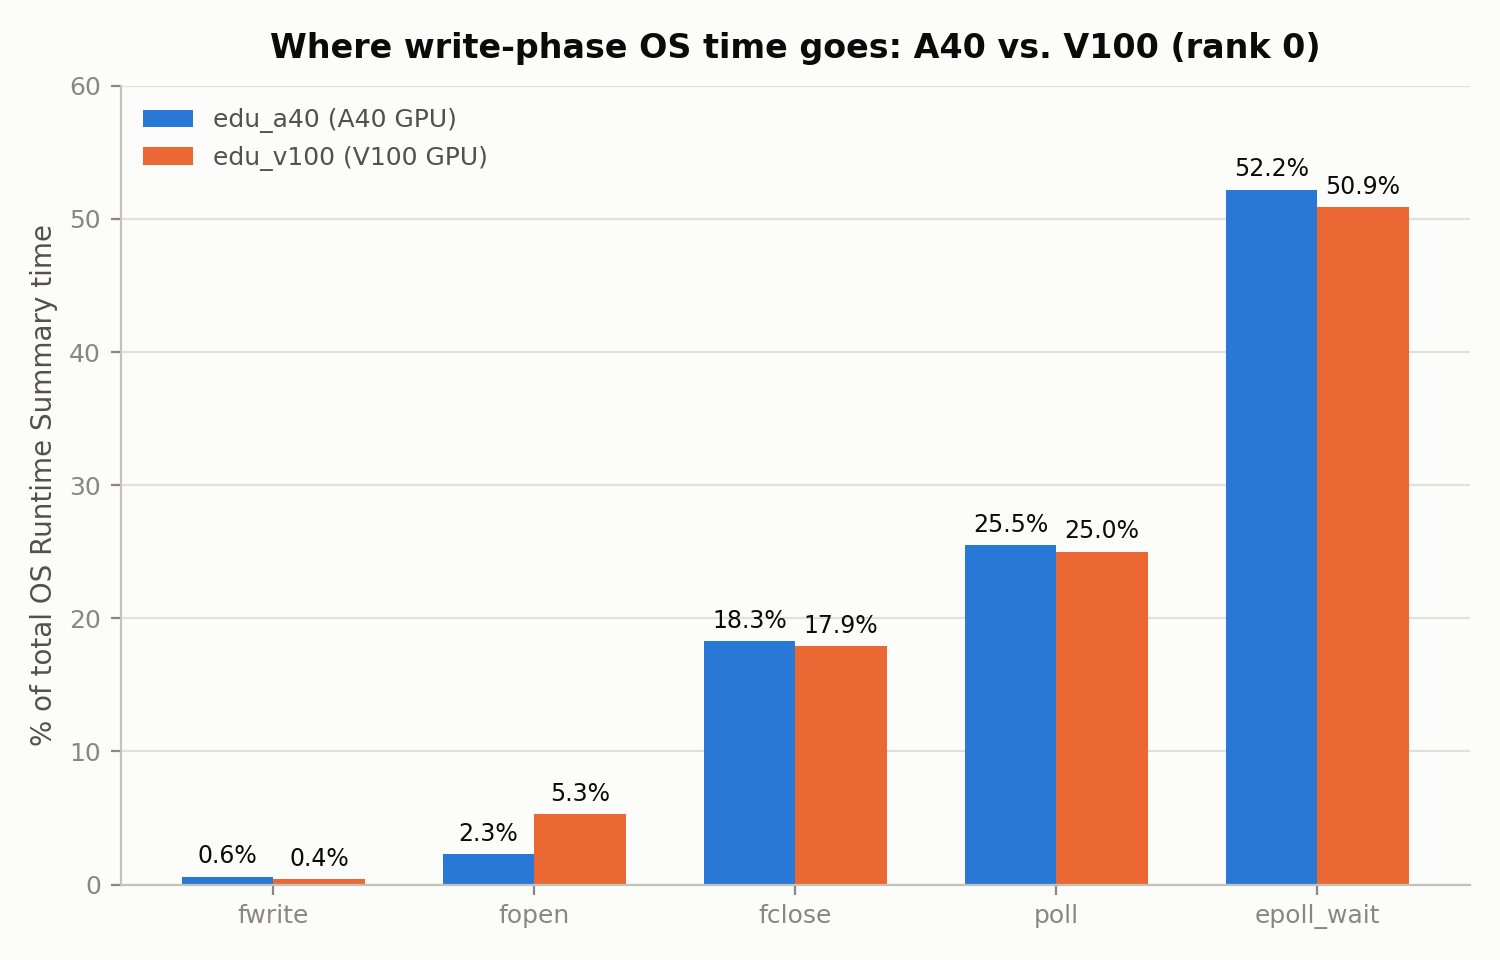
\includegraphics[width=0.6\textwidth]{../src/Davide/Final/Latex/figures/nsys_os_runtime_breakdown.png}
    \caption{OS Runtime Summary breakdown (rank 0), \texttt{edu\_a40} vs.\ \texttt{edu\_v100} -- nearly identical despite very different GPU hardware.}
    \label{fig:nsys}
\end{figure}

\subsection{OpenMP thread scaling and CUDA block size}
Figure~\ref{fig:thread} sweeps OpenMP thread count 1--32 at $M=4096$ (the
full logical-core range of one \texttt{edu\_a40} rank, $96/3$). Both the
full-pipeline and \texttt{compute\_next}-only curves are essentially
flat, never exceeding $\sim$1.2$\times$ speedup, with compute-only
plateauing by 2 threads and staying flat through 32. This is consistent
with the 5-point stencil being memory-bandwidth-bound rather than
compute-bound (4 loads, 1 store, few FLOPs per point) -- a small number
of threads already saturates available memory bandwidth. We also
considered an alternative explanation -- that \texttt{compute\_next}
forking a fresh OpenMP thread team on every one of 300 calls/rank could
plateau this curve through fork/join overhead alone, independent of
memory bandwidth -- and ruled it out with VTune Hotspots at $M=4096$:
\texttt{gomp\_team\_barrier\_wait\_end} does not appear among the top
hotspots at either 4 or 32 threads (unlike part 1's profile, where it was
79.4\% of CPU time), and \texttt{compute\_next}'s own CPU time is flat
across that range (3.43s at 4 threads vs.\ 3.21s at 32) rather than
growing with team size. This contrasts
with part 1's own OpenMP results, which showed real scaling at large
thread counts, mainly because part 1 tested $M$ up to 15000 -- large
enough for the stencil's absolute cost to be interesting on its own,
with no competing GPU-bound stage.

\begin{figure}[h]
    \centering
    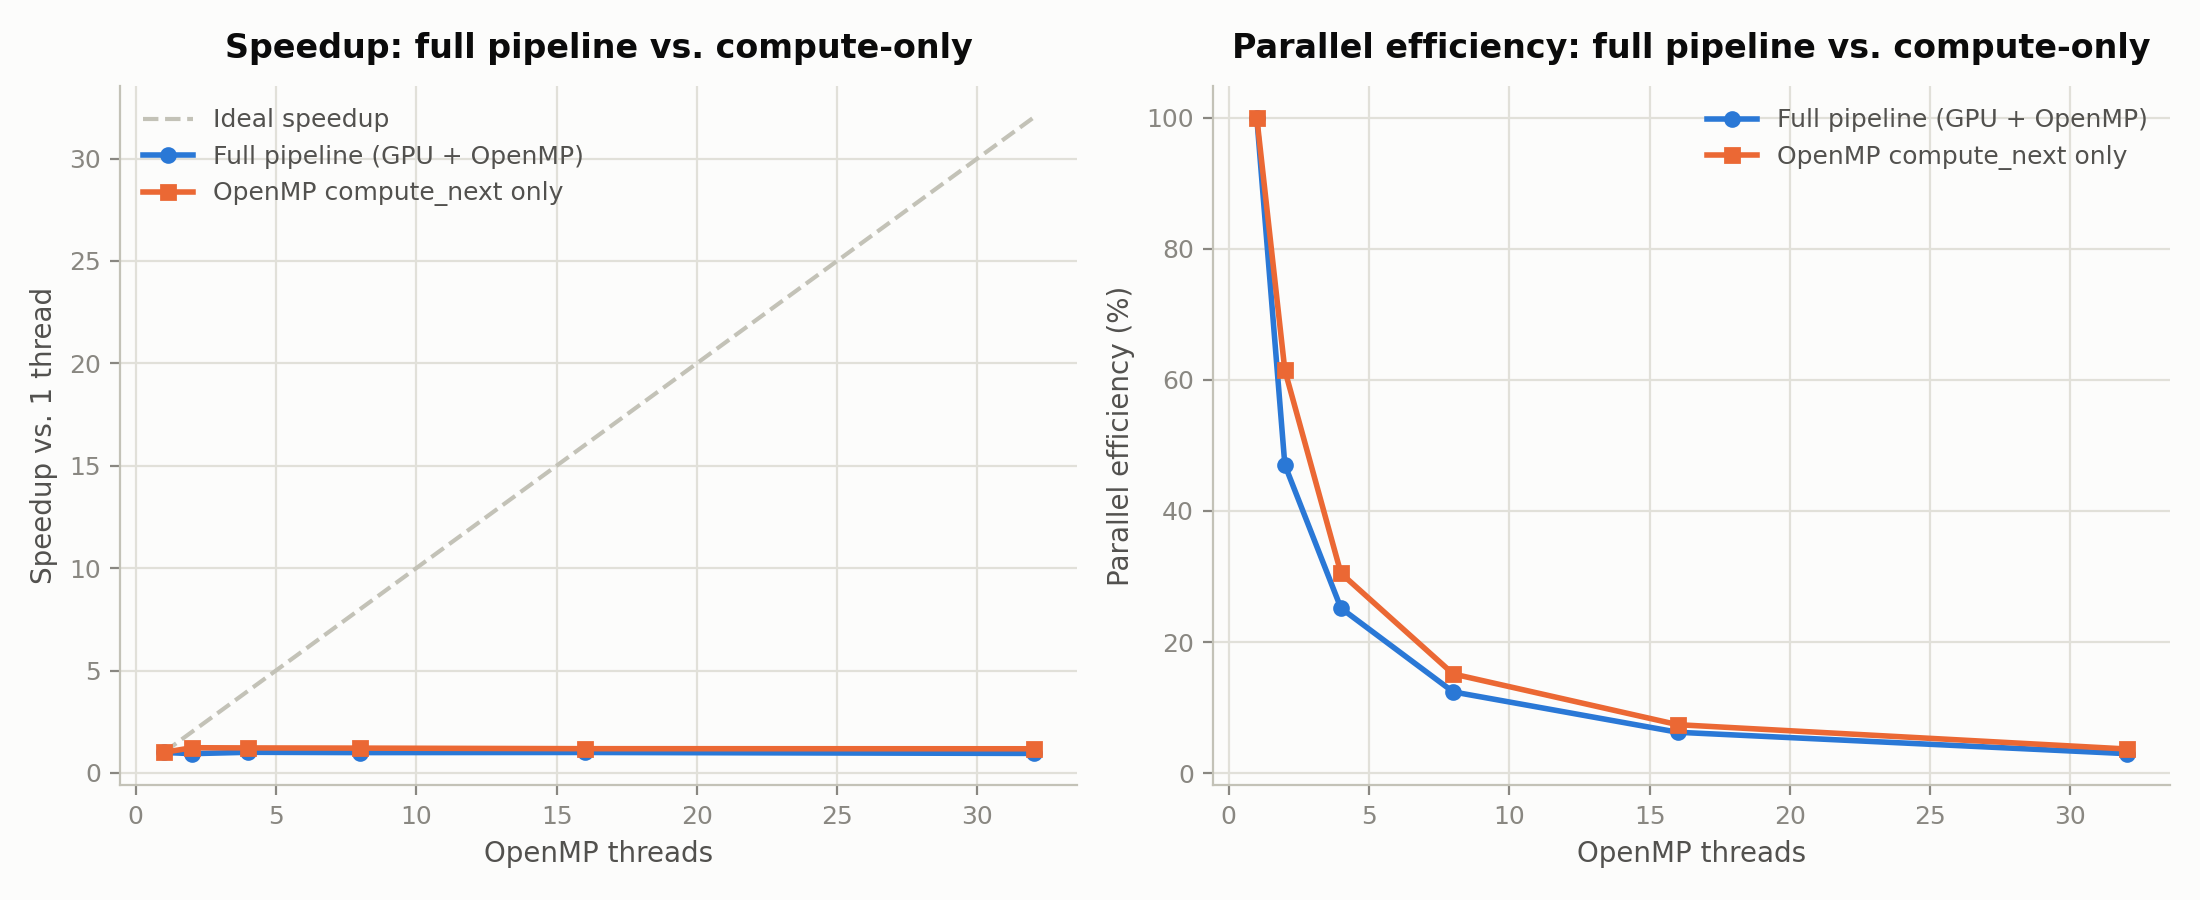
\includegraphics[width=0.68\textwidth]{../src/Davide/Final/Latex/figures/thread_sweep_speedup_efficiency.png}
    \caption{Speedup and efficiency vs.\ OpenMP thread count at $M=4096$, full pipeline vs.\ compute-only.}
    \label{fig:thread}
\end{figure}

Figure~\ref{fig:block} sweeps the CUDA kernel's threads-per-block at
$M=4096$: time decreases roughly monotonically as block size grows,
worst at 32 threads/block ($\sim$83s average) and best at 1024
($\sim$73s, $\sim$12\% faster), with only a minor plateau between 128
and 512. Since Nsight Compute (the tool that would report actual
occupancy) is unavailable on this cluster, we do not have a
profiler-level explanation for this trend, only the timing result
itself -- the most we can say is that fewer, larger blocks amortize
per-block launch and scheduling overhead across more threads. A smaller,
noisier earlier sweep at $M=1024$ (not shown) trended the opposite way
at the high end, so we do not treat this shape as independently
confirmed and report only the $M=4096$ result.

\begin{figure}[h]
    \centering
    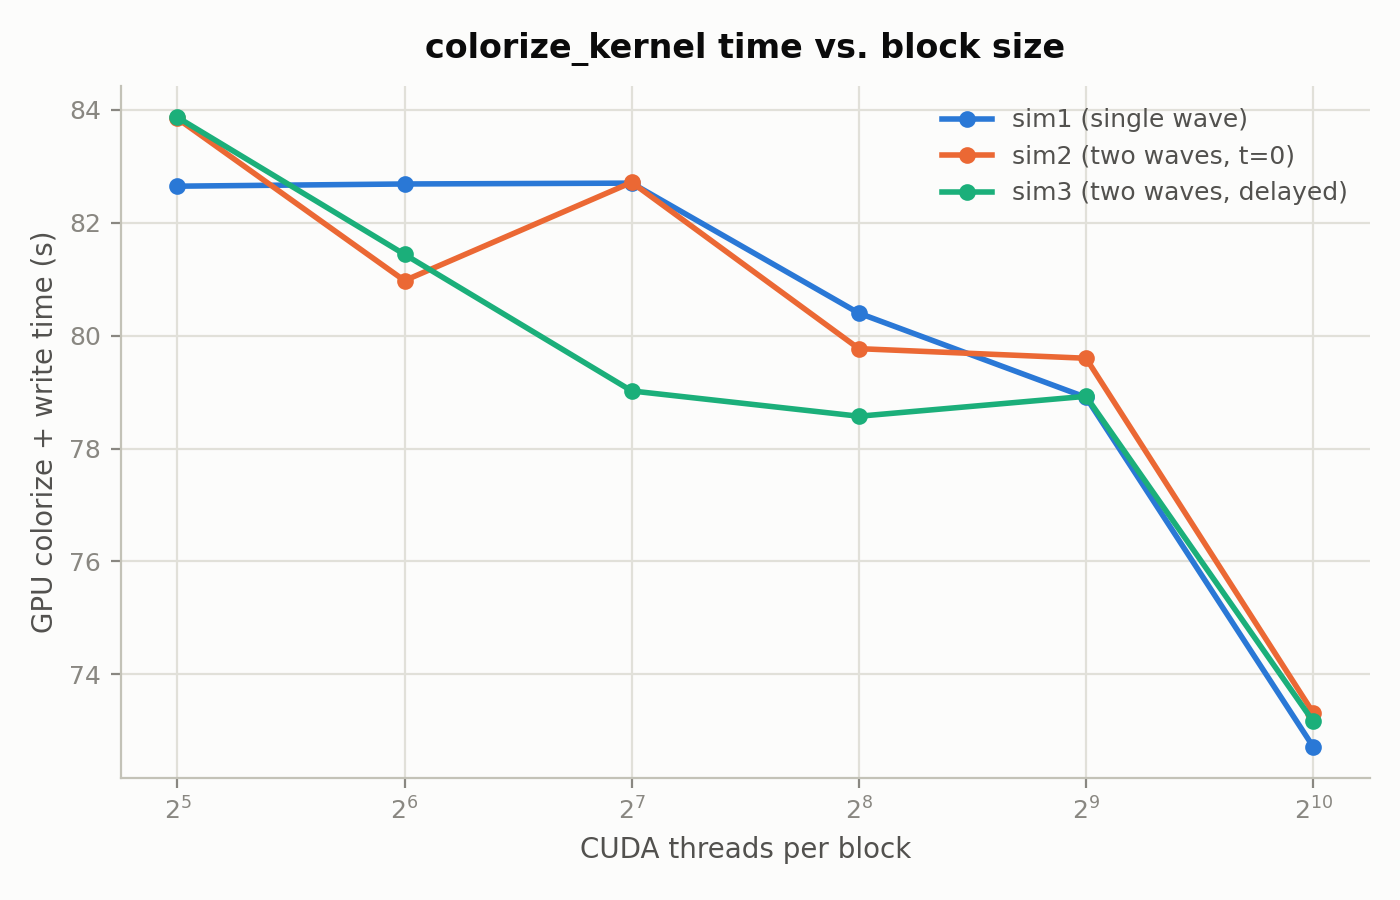
\includegraphics[width=0.52\textwidth]{../src/Davide/Final/Latex/figures/blocksize_sweep_kernel_time.png}
    \caption{GPU colorize+write time vs.\ CUDA threads-per-block, $M=4096$.}
    \label{fig:block}
\end{figure}

\subsection{GPU contention across execution modes}
\label{sec:contention}
Section~\ref{sec:phase} showed disk writes dominate; this raises the
question of how much the design choice of sharing one GPU across 3
ranks actually costs. We compared four execution modes at identical
parameters ($M=2048$, 50 steps, 4 threads), isolating sim1's workload
in each: \texttt{solo} (1 rank, exclusive GPU), \texttt{shared} (the
normal 3-rank/1-GPU run), \texttt{distributed} (3 ranks, 3 dedicated
GPUs on one node, \texttt{--gres=gpu:3}), and \texttt{multinode} (3
ranks on 3 separate nodes, one dedicated GPU each, communicating over
the cluster's Infiniband fabric \cite{sanchezmpitopo}). Results
(Figure~\ref{fig:contention}): \texttt{solo} 9.47s, \texttt{shared}
20.84s, \texttt{distributed} 21.25s, \texttt{multinode} 18.76s.

Two findings. First, dedicating a GPU per rank alone
(\texttt{distributed} vs.\ \texttt{shared}) makes no reliable difference
at all -- \texttt{distributed} is actually $\sim$2\% \emph{slower} here,
well within run-to-run noise rather than a real effect either way --
GPU compute-engine time-slicing is not the bottleneck. Second,
\texttt{solo} is dramatically faster than every multi-rank mode (roughly
half the time, $\sim$50--55\% less depending on which mode it's compared
against), which Section~\ref{sec:phase}'s finding
explains directly: \texttt{shared} and \texttt{distributed} both have 3
ranks writing frames \emph{concurrently} to the same node; \texttt{solo}
is the only mode with exactly one writer at a time, anywhere.
\texttt{multinode} sits in between ($\sim$10\% faster than
\texttt{distributed}) by removing host-local contention (memory bus,
PCIe root complex) but not, most plausibly, a deeper one: all three
nodes most likely still write to the same shared, network-attached
storage behind every node's home directory (per the cluster's own
documentation, though not measured directly here) -- the best available
explanation for why multinode sits closer to \texttt{shared} than to
\texttt{solo}. The dominant contention in this workload is concurrent
I/O, not GPU compute-engine sharing -- consistent with
Section~\ref{sec:nsys}'s \texttt{fclose}-dominated OS Runtime profile.

\begin{figure}[h]
    \centering
    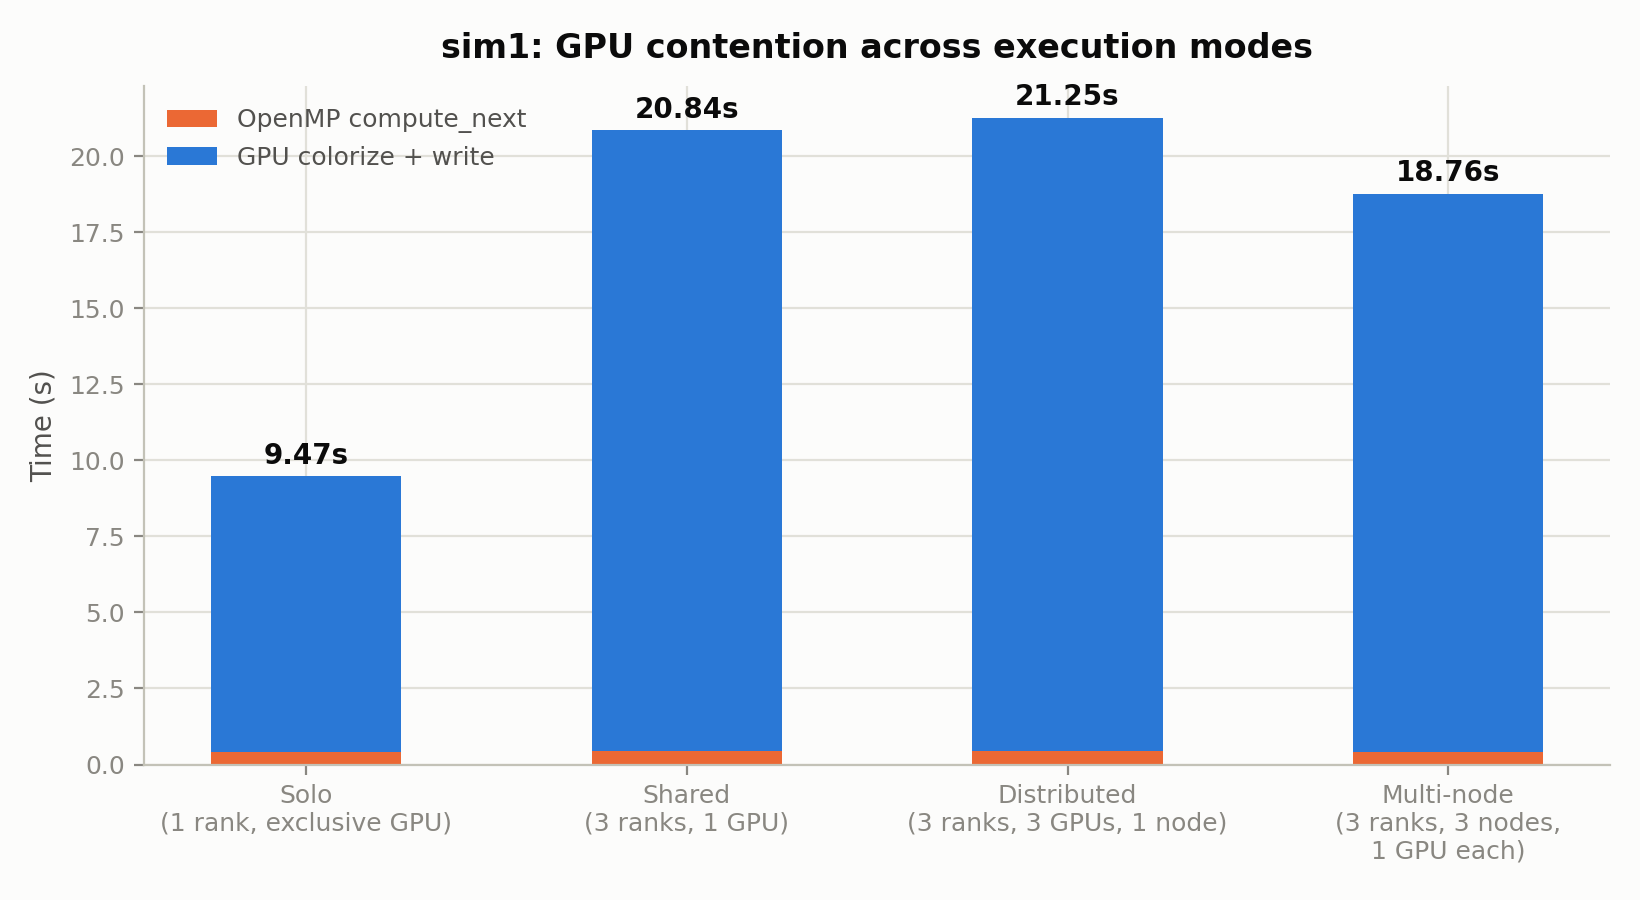
\includegraphics[width=0.6\textwidth]{../src/Davide/Final/Latex/figures/contention_sweep_solo_vs_shared.png}
    \caption{sim1's execution time across four GPU/node sharing configurations, identical workload.}
    \label{fig:contention}
\end{figure}

\subsection{Conclusions}
The dominant cost in this pipeline is not GPU compute (colorization
kernel: $\sim$1\% of frame time) nor CPU compute
(\texttt{compute\_next}: $\sim$2\%), but per-frame file I/O, specifically
whatever happens at \texttt{fclose} time rather than the write itself --
confirmed consistent across two GPU generations and reflected directly
in the GPU-sharing contention results: sharing the GPU across ranks
costs almost nothing, while sharing the filesystem costs a great deal.
This is the throughline of the whole investigation -- every optimization
decision was made only after measuring, not assumed from the physics
alone. Parallelizing the ASCII-formatting step was considered and
rejected once the phase breakdown showed it was $\sim$4\% of
\texttt{color\_time}, not worth the added complexity. Per-frame adaptive
color scaling was adopted only after raw pixel data confirmed a fixed
scale reads as pale almost immediately, since a 2D wave's peak amplitude
falls off geometrically with distance from the source on top of
$\gamma$-damping. And the GPU-sharing question itself was settled by
directly comparing four execution modes rather than assumed from GPU
specifications -- the result (I/O-bound, not compute-bound) held
consistently across every measurement in this report.
